%%%%%%%%%%%%%%%%%%%%%%%%%%%%%%%%%%%%%%%%%
% Journal Article
% LaTeX Template
% Version 1.4 (15/5/16)
%
% This template has been downloaded from:
% http://www.LaTeXTemplates.com
%
% Original author:
% Frits Wenneker (http://www.howtotex.com) with extensive modifications by
% Vel (vel@LaTeXTemplates.com)
%
% License:
% CC BY-NC-SA 3.0 (http://creativecommons.org/licenses/by-nc-sa/3.0/)
%
%%%%%%%%%%%%%%%%%%%%%%%%%%%%%%%%%%%%%%%%%

%----------------------------------------------------------------------------------------
%	PACKAGES AND OTHER DOCUMENT CONFIGURATIONS
%----------------------------------------------------------------------------------------

\documentclass[twoside,twocolumn]{article}
\usepackage{blindtext} % Package to generate dummy text throughout this template 
\usepackage{gensymb}
\usepackage{mhchem}
\usepackage{natbib}
\usepackage{setspace}
\setlength{\bibsep}{-0.6pt}
\bibliographystyle{agsm}
%\bibliographystyle{abbrv}
%\bibliographystyle{apalike}
%\bibliographystyle{ksfh_nat}
%\bibliographystyle{agsm}
\usepackage[sc]{mathpazo} % Use the Palatino font
\usepackage[T1]{fontenc} % Use 8-bit encoding that has 256 glyphs
\linespread{1} % Line spacing - Palatino needs more space between lines
\usepackage{microtype} % Slightly tweak font spacing for aesthetics

\usepackage[english]{babel} % Language hyphenation and typographical rules
\usepackage{float}% use h to force table into location
\usepackage{longtable} %let table span
\usepackage[hmarginratio=1:1,top=25mm,columnsep=10pt,total={7.5in, 9in}]{geometry} % Document margins
\usepackage[hang, small,labelfont=bf,up,textfont=it,up]{caption} % Custom captions under/above floats in tables or figures
\usepackage{booktabs} % Horizontal rules in tables
\usepackage{graphicx}
\graphicspath{ {./Figures/} }
\usepackage{lettrine} % The lettrine is the first enlarged letter at the beginning of the text
\usepackage{subcaption} %sub-figures
\usepackage{wrapfig}

\usepackage{enumitem} % Customized lists
\setlist[itemize]{noitemsep} % Make itemize lists more compact

\usepackage{abstract} % Allows abstract customization
\renewcommand{\abstractnamefont}{\normalfont\bfseries} % Set the "Abstract" text to bold
\renewcommand{\abstracttextfont}{\normalfont\small\itshape} % Set the abstract itself to small italic text

\usepackage{titlesec} % Allows customization of titles
\renewcommand\thesection{\Roman{section}} % Roman numerals for the sections
\renewcommand\thesubsection{\roman{subsection}} % roman numerals for subsections
\titleformat{\section}[block]{\large\scshape\centering}{\thesection.}{1em}{} % Change the look of the section titles
\titleformat{\subsection}[block]{\large}{\thesubsection.}{1em}{} % Change the look of the section titles

\usepackage{fancyhdr} % Headers and footers
\pagestyle{fancy} % All pages have headers and footers
\fancyhead{} % Blank out the default header
\fancyfoot{} % Blank out the default footer
\fancyhead[C]{Imperial College London $\cdot$  December 2020 	$\cdot$ Project 72} % Custom header text
\fancyfoot[RO,LE]{\thepage} % Custom footer text

\usepackage{titling} % Customizing the title section

\usepackage{hyperref} % For hyperlinks in the PDF

%----------------------------------------------------------------------------------------
%	TITLE SECTION
%----------------------------------------------------------------------------------------

\setlength{\droptitle}{-4\baselineskip} % Move the title up

\pretitle{\begin{center}\Huge\bfseries} % Article title formatting
%\posttitle{\end{center}} % Article title closing formatting
\title{Synthesis and Optimisation of Novel Corn Starch Superhydrophobic CaCO$_3$ Films} % Article title
\author{%
\text{Dhylan Mistry \& Shav Vimalendiran }%\thanks{Can thank Vikram here} 
\\[1ex] % Your name
\normalsize \emph{Department of Chemical Engineering, Imperial College London}\\ % Your institution
%\normalsize \href{mailto:john@smith.com}{john@smith.com} % Your email address
%\and % Uncomment if 2 authors are required, duplicate these 4 lines if more
%\textsc{Jane Smith}\thanks{Corresponding author} \\[1ex] % Second author's name
%\normalsize University of Utah \\ % Second author's institution
%\normalsize \href{mailto:jane@smith.com}{jane@smith.com} % Second author's email address
}
\date{} % Leave empty to omit a date
\renewcommand{\maketitlehookd}{%
\begin{abstract}
\noindent Nature is an inexhaustible source of inspiration; non-wetting lotus leaves have sparked considerable interest in the scientific community over the past decades. Superhydrophobic films have a wide range of industrial applications, but it is equally as important to mitigate environmental damage whenever pursuing these applications. Herein, we report the preparation of superhydrophobic composite coatings with an eco-friendly technique. The possibility of removing harmful solvents and non-bioderived polymers are investigated using precipitated calcium carbonate as the substrate (which can also be derived from eggshells), stearic acid as the surface modifying agent and corn starch as the binder. Following characterisation, the novel films show promising mechanical and superhydrophobic properties. An optimised formulation using corn starch with 50\%w/w hydrophobic powder and 5.5\%w/w stearic acid is presented as a statistically significant replacement for polyethylene/toluene films in terms of practical durability as well as superhydrophobicity (contact angle of 154.8$^\circ$ $\pm$ 4.7 $^\circ$ vs 151.7 $^\circ$ $\pm$ 1.5 $^\circ$ for polyethylene/toluene and optimised formulation respectively). 
%Eco-friendly composite coatings were prepared using an in development hydrophobic powder of precipitated calcium carbonate functionalised with stearic acid and starch as the potential binder. The films show promising mechanical and hydrophobic properties and is a candidate for [real life use of it].After using stearic acid to modify PCC, the dip-coating method was used to prepare the corn starch composite films. Physical, mechanical, hydrophobic and thermal properties were characterized using a goniometer, optical microscopy, and dynamic vapour sorption. The results showed that:

%\noindent Hydrophobicity can improve the usability and functionality of materials in humid condition, enhancing the hydrophobic behavior of starch films is of inportance. 


%\noindent In this project, the possibility of removing harmful solvents and non-bioderived polymers are investigated to produce superhydrophobic coatings from calcium carbonate intended to be derived from eggshells. The coating was manufactured by... 
\end{abstract}
}

%----------------------------------------------------------------------------------------

\begin{document}
% a
% Print the title
\maketitle

%----------------------------------------------------------------------------------------
%	ARTICLE CONTENTS
%----------------------------------------------------------------------------------------

\section{Introduction}
\lettrine[nindent=0em,lines=2]{T}he origins of superhydrophobicity research are traced to \cite{ollivier_1907}  where perfect sphere beads of water were observed on toxic arsenic trioxide and soot surfaces. Hydrophobicity arises on a surface from a lack of attractive forces causing water to 'repel' off the surface (\cite{Hydrophobicreview}).The self cleaning and superhydrophobic 'lotus effect' has fascinated researchers; research in the area has been re-energised by the discovery that \textbf{low surface energy} from epicuticle wax crystals as well as \textbf{surface roughness} from papillae are fundamental to the phenomena. The growth in interest is also spurred by its applications particularly in acid- rain building protection, self-cleaning surfaces and rust protection (\cite{LATTHE201952},\cite{SHSreview}). 
\par It is understood that low surface energy causes water droplets to bead up and potentially roll off. If the surface energy is high, water will spread out on the surface (e.g. glass) due to favourable interactions. The degree of hydrophobicity is characterised by the Water Contact Angle (WCA). An angle above 90$^\circ$ is hydrophobic and above 150$^\circ$ is superhydrophobic (\cite{SHSreview},\cite{ECOSHS}). 
\par To minimise surface energy, silanated compounds, particularly fluoroalkylsilanes, gain the most attention due to the greatest minimisation in surface energy. Despite being very effective, their high cost and toxicity to the environment has incentivised researchers to seek alternatives. Hence, it was discovered that the roughened metallic surface of CaCO$_3$ develops superhydrophobicity when functionalised with surfactants (\cite{demjen}). Fatty acids have been utilised due to commercial availability and reduced toxicity to the environment (\cite{SHENG20061983},\cite{HuDeng}, \cite{Cao}).The carboxylic acid head (hydrophilic)  chemisorbs onto the CaCO$_3$ surface seen in Figure \ref{calcium}, with the aliphatic tail orientated to provide surface hydrophobicity as well as physisorption from multiple layers of fatty acid (\cite{Kokkinis_2017}). 

\begin{figure}[h!]
\centering
  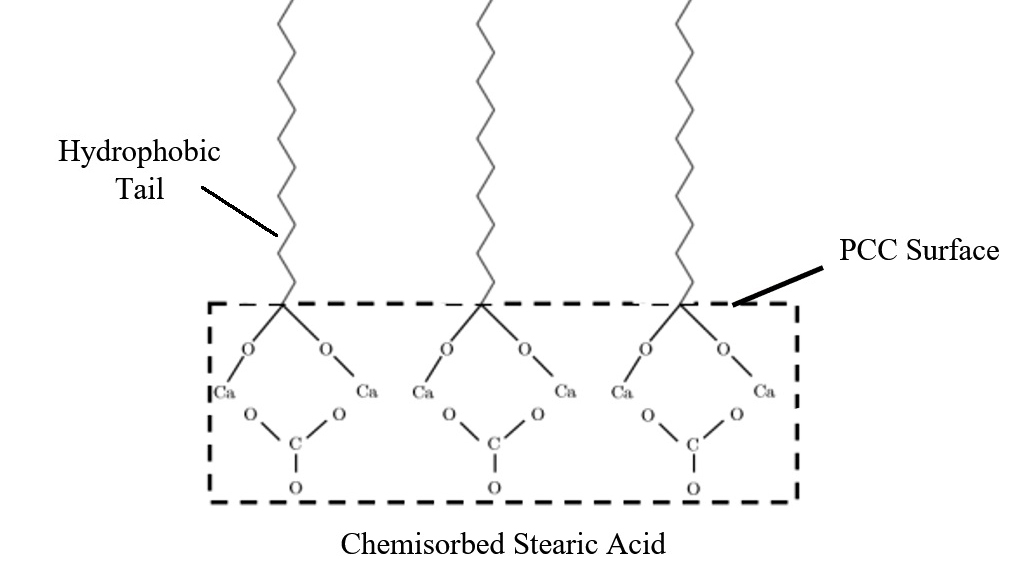
\includegraphics[width=0.35\textwidth]{Sections/Figures/SAFunctionalised4.jpg}
  \caption{Monolayer chemisorbed fatty acid functionalised CaCO$_3$ }\label{calcium}
\end{figure}

To form a monolayer, ball milling, pestle and mortar milling as well as wet methods such as a hot aqueous slurry have been used (\cite{Cao},\cite{DeArmritt}). Pestle and mortar dry milling was used in this project due to simplicity, no solvent and restricted access to laboratory equipment for ball milling. 

Stearic acid and Oleic acid, derived from sources such as cocoa butter and olives respectively, have been used as eco-surfactants and yielded successful SHP\footnote{Superhydrophobic Powder} using the mechano-chemistry technique rather than the wasteful solvent approach (\cite{deepika}). Stearic acid is one of the most suitable surfactants for calcium carbonate as it provides maximum surface coverage (\cite{gilbert_petiraksakul_mathieson_2001}). The powder was further optimised from hydrophobic to superhydrophobic with 2\%w/w stearic acid (\cite{Vatsal}.). Superhydrophobicity can also be attributed to the hierarchical structure of CaCO$_3$ that provides surface roughness as seen by SEM imaging (\cite{zhang_hierarchial}). The source of calcium carbonate has evolved from limestone and now can be derived from natural waste products such as eggshells (\cite{thailandshells}), and seashells (\cite{fang_2019}) enhancing sustainability.
\par Besides the superhydrophobicity of the powder,  there was an additional challenge of producing a sustainable paint (binder solution) so that a homogeneous coating can be practically applied. Due to environmental concerns, starch has received a lot of attention; as a natural biodegradable biopolymer, it is a promising candidate to replace the petroleum-derived materials currently in use. Starch already boasts a wide range of uses in industry - it is used in cosmetics, textiles, pharmaceuticals and fuels amongst others (\cite{kaur_ariffin_bhat_karim_2012}).  Amongst the candidates for petroleum replacement, starch is one of the most encouraging due to its diversity, film forming properties, availability, cost-effectiveness, and ease of handling (\cite{dufresne}, \cite{Caoprep}).  
\par Starch has been obtained from various botanical sources; as a consequence of its numerous sources, starch itself is a diverse polymer with different shapes, sizes, structures and chemical properties (\cite{smith_2001}). Starch contains two macro molecules: amylose (linear) and amylopectin (branched), with varying compositions allowing diverse physico-chemical properties of starch-based films. Corn Starch (Zea mays L.) was sourced with  28\% w/w amylose content  and a gelatinisation temperature of above 59.7 °C (\cite{luchese_spada_tessaro_2017}). Gelatinisation was essential to mitigate issues with cracking, hygroscopicity and non-continuous/inconsistent film formation (\cite{ZOBEL1984285}). Corn Starch was chosen as a starting point due to its low-cost and relatively high amylose content contributing to improved film flexibility, continuity and strength that occurs on cooling after gelatinisation (\cite{Amylosebenefit}).
\par Starch repeating units feature three free OH groups on each glycoside ring, making the molecule strongly hydrophilic. The OH groups make starch a promising binder due to H bonding with glass. Despite improving the binding ability, various starch hydrophobic functionalisation processes were reviewed to counteract the inherent hydrophilicity which reduces the hydrophobicity of the coating (\cite{wang}). \cite{jiang_dai_qin_xiong_sun_2016} demonstrated short-chain amylose starch modification in ethanol solution using 2-Octen-1-yl Succinic Anhydride (OSA) to produce amphiphilic OSA-starch-nanoparticles (OSA-SNP’s). The hydrophobicity of OSA-SNP’s increased with the degree of substitution as the OH groups on starch molecules were replaced by hydrophobic OSA groups. \cite{yu_jiang_zheng_cao_hou_xu_wang_jiang_pan_2019} formulated OSA-SNP powders which were pressed to obtain tablets; the starch modification had little effect on the particle size or morphology of starch, but increased the contact angle significantly, from 25.4° to 70.1°. The amphipathicity of modified starch polymers would increase the hydrophobicity of films over those that retained OH groups e.g.  unmodified corn starch. The OSA-Corn starch films were created using a modified method as described by \cite{OMSProcess}. 
\par The addition of inorganic tetraethylorthosilicate (TEOS) can also improve hydrophobicity of starch based-films (\cite{TEOS}) by the synergism of the components to form a starch-inorganic hybrid material. An adapted procedure was undertaken to prepare films by dip-coating with hydrolysis and condensation of TEOS in situ under a controlled pH, as demonstrated by \cite{TEOS}. 
\par Water molecules can also act as a plasticiser for hydrophilic polymers. \cite{wang_gu_hong_cheng_li_2011} demonstrated how the addition of silica nanoparticles at 10\% w/w corn starch not only increased shear strengths of starch-based binder but also increased the water resistance by 20.2\%, something invaluable for industrial applications in humid environments. Starch films incorporating silica nanoparticles were also investigated.

Producing superhydrophobic coatings that not only have a high WCA but are more sustainable is still a trending topic. (\cite{ECOSHS}). This year, water based PVA films have been produced (\cite{rewritable}) with 160° WCA as well as nano-CacO$_3$  films using Ethanol as a solvent but with 107° WCA. (\cite{syafiq_vengadaesvaran_ahmed_rahim_pandey_bushroa_ramesh_ramesh_2020}). There is limited research into using corn starch to develop superhydrophobic coatings. A recent superhydrophobic starch coating developed used expensive 80\% amylose corn starch , PDMS, Montmorillonite and a multi-step application process involving spraying/curing(\cite{chen_liu_yu_duan_ji_chen_2020}). Other superhydrophobic coatings developed utilise the developed SHP from CaCO$_3$ but use plastics such as Polyethylene and Polystyrene with a toluene solvent (\cite{Vatsal}).  Hence, there is a clear opportunity to combine the promising SHP with corn starch to produce superhydrophobic films. 

\subsection{Objectives}

This project aims to investigate the feasibility of replacing the  most recently optimised superhydrophobic coating using PE and Toluene (\cite{fang_2019}) with starch to produce a stable, homogenous film thus reducing harmful solvents and plastics in the environment. Various starch coatings will be produced in order to optimise the formulation. The efficacy of hydrophobic starches (see introduction) will be explored and quantified. The proposed coating must be able to be dried at ambient conditions and be applied simply by dip-coating.  The hydrophobic characteristics and durability of developed formulations will be compared and contrasted to the current formulation. 
\newpage
\subsection{Theory of Wetting Phenomena} 
Water contact angle (CA) is defined by the intersection of the three-phase boundary between solid, liquid and vapour. This is commonly described using Young’s equation:
\begin{equation}
\label{Young}
\gamma_s_v = \gamma_s_l + \gamma_l_v cos \theta_i
\end{equation}1
Here, $\gamma_s_v$, $\gamma_s_l$ and $\gamma_l_v$ denote the surface tensions of solid-vapour, solid liquid and liquid vapor respectively. $\theta_i$ denotes the ‘equilibrium’ CA on an \emph{ideal} surface i.e. one that is smooth, inert, homogeneous and nonporous. \cite{wenzel_1936} proposed an expression for the apparent equilibrium CA $\theta_w$ to account for surface roughness, as a function of roughness factor $r_f$
\begin{equation}
\label{Young}
cos \theta_w = r_f cos \theta_i
\end{equation}
This is valid when there is no gas trapped in between the droplet and crevices of the surface. When gas is trapped,  the Cassie and Baxter model is used: 
\begin{equation}
\label{Young}
cos \theta_c = \sigma (1+ cos \theta_i) -1
\end{equation}
Here the apparent CA ($\theta_c$) is a function of the relative fractional area of solid in contact with air, $\sigma$, and $\theta_i$ (\cite{cassie_baxter_1944}). In this model, the more air trapped between the liquid-solid interface, the higher the contact angle. 

However, static contact angle measurements alone aren’t sufficient to fully characterise a surface as using the average static CA neglects the irregularities of a real surface. One static, metastable CA only designates an angle within the range of contact angles possible between the advancing, $\theta_A$, and receding, $\theta_R$, contact angles; reporting the dynamic contact angles are therefore important criteria to further characterize the hydrophobicity of our film surfaces (\cite{gao_mccarthy_2006}). Hysteresis is the term used to describe this range between advancing and receding contact angles; it originates from and can indicate the properties that cause a surface to differ from the ideal, such as surface inhomogeneity and roughness. 


%\lettrine[nindent=0em,lines=3]{L} orem ipsum dolor sit amet, consectetur adipiscing elit.
%\blindtext % Dummy text

%\blindtext % Dummy text

%------------------------------------------------
\section{Method \& Materials}
\subsection{Materials} 
\textbf{Precipitated CaCO$_3$(PCC):} Fisher Scientific (minimum assay 98\%) containing calcite polymorph.
\textbf{Stearic Acid:} C$_1_7$H$_3_5$COOH from BDH Chemicals Ltd. as a GPR with a solubility of 0.57mg/l at 25$^\circ$C \cite{stearic}. 
\textbf{DI Water:} used in all experiments.
\textbf{Ethanol:} C$_2$H$_5$OH absolute (99.97\% minimum assay) from VWR chemicals. Second most widely used industrial solvent due to lower toxicity than other alcohols and possibility for bio-derivation. \textbf{Toluene:} C$_7$H$_8$ as ACS reagent from VWR Chemicals (minimum assay 99.9\%). Extremely flammable with a flashpoint of 4.4$^\circ$C.
\textbf{Corn Starch:} (C$_6$H$_1_0$O$_5$)$_n$ from Sainsbury's. Formula is the repeat unit for the ${\alpha}$ 1,4 linkages.  
\textbf{PE:} (C$_2$H$_4$)$_n$ as ACS reagent from BDH ltd. UK.
\textbf{TEOS:} from Sigma-Aldrich (minimum assay 99\%). \textbf{Hydrophobic fumed silica:} 'Aerosil \textsuperscript \textregistered  R 972 treated with DDS' from Evonik, Germany. BET Surface Area of 90-130 m$^2$/g with $d_p$=16-20nm. \textbf{OSA:} (2-Octen-1-ylsuccinic anhydride) from Sigma-Aldrich (minimum assay 97\%). \textbf{NaOH} ACS reagent from VWR Chemicals (minimum assay 99.6\%). Utilised for pH adjustment in both TEOS (\cite{TEOS}) and OSA (\cite{OMSProcess}) procedures.
\subsection{Formulation Methodology}
\begin{table} [H]
\centering
\begin{tabular}{llr}
\toprule
Key & Formulation\\
\midrule
A   & PE+Toluene              \\ 
B   & 5g Starch               \\ 
Bb  & 5g starch,Drying at 60 $^\circ$C, 700mBar \\ 
C   & 5g starch/0.286g silica \\ 
D   & 5g Starch/2gTEOS        \\ 
E   & 5g OMS Powder           \\ 
\bottomrule
\end{tabular}
\caption{Formulation naming key. '\textbf{A-40-2.5}' for example corresponds to formulation A with 40\%w/w hydrophobic powder and 2.5\%w/w stearic acid.}
\label{Key}
\end{table}

\textbf{Functionalised Powder:} prepared by addition of desired PCC:SA to a stainless steel pestle and mortar and milled for 10 mins to form hydrophobic powder (\cite{fang_2019}). 
\newline \textbf{Octenyl Modified Starch (OMS) Powder:} 20g corn starch was suspended in 100ml of DI water, pH adjusted via addition of 3\%w/w NaOH and stirred (MS-H280-Pro stirrer) at 25 $^{\circ}$C for 10 mins. 3ml of OSA was diluted in 1:5 OSA to Ethanol mixture and mixed at 35 $^{\circ}$C for 2 hrs. The mixture was filtered using 'Whatman \textsuperscript \textregistered  Grade 1 (11 $\mu$m) filter paper and washed with 500ml distilled water. The residue was placed into glass petri dishes, dried in a vacuum oven at 60 $^\circ$C, 700mbar for 24 hr and then shattered into powder. (\cite{OMSProcess}, \cite{PowderShatter})
\newline \textbf{Paint formulations:} Followed 2-step method presented by \cite{tzouganatos_2015}.  This involved binder solution preparation followed by addition of hydrophobic powder. All formulated paints were dip coated onto Glass Microscopic Slides (1.0mm thick, 25mm x 75mm) to produce 4 samples. All samples, unless otherwise stated, were dried at ambient conditions in the fume-cupboard for 72 hrs.  
\par \textbf{A:} 2\%w/v of PE was dispersed in Toluene and heated under reflux at 90$^{\circ}$C for 20 minutes.  40\%w/w of 2.5\% w/w SA functionalised powder was added and mixed for a further 25 minutes at 90$^{\circ}$C.  
\par \textbf{B:} 5 g of corn starch dispersed in 100ml 1:1 Ethanol:DI Water was covered with parafilm to avoid solvent loss and mixed at 70 $^{\circ}$C for 20 minutes to achieve starch gelatinisation (\cite{5starch}, \cite{StarchGel}). Temperature was maintained by both a thermometer as well as a temperature probe from the stirrer. Hydrophobic powder was rapidly added, recovered with parafilm and stirrer speed increased to mix for 5 minutes. \textbf{Bb} was an exception and had controlled drying (see table \ref{Key}). \textbf{Adaptations for C and E} were 0.286g of nano-silica addition for C added with the 5g of cornstarch, and for E 5g of OMS replaced 5g of corn starch. 
\par \textbf{D}: 5g of corn starch was dispersed in the same way as B for 20 minutes. The filmogenic solution was cooled to 40$^{\circ}$C followed by a pH adjustment to 9 with NaOH. The pH was verified with 'Fisherbrand \textsuperscript \textregistered pH indicator sticks' and immediately followed by the slow addition of 2ml TEOS by syringe. The mixture was mixed for 1 hour at 40$^{\circ}$C and the functionalised powder rapidly added. The mixture was left to mix for a further 10 minutes.
\subsection{Contact Angle Characterisation Methodology}
Quantitative characterization of surface wettability was carried out through static CA measurement as well as sessile-droplet method for Hysteresis. Measurements were performed digitally on a ramé-hart advanced goniometer (590-u1). Accurate droplet volume dispensing was achieved using a ramé-hart Automated Dispensing System (100-22). 
\par The dip-coated slides were placed onto the projection stage with sufficient backlight and the steel needle dropper was adjusted and focused in the frame before the stage was analysed using DROPimage Advanced software. For static CA measurements, a 10 $\mu$L droplet of DI water was placed on the surface and 100 measurements with a time interval of 0.01s were taken from the side profile. Measurements on each slide were performed in three locations to test surface homogeneity, and repeated for 2 separate slides to indicate reproducibility of the dip-coating method.
\par For the Sessile-droplet method,  the needle was used to slowly dispense a droplet of 20 $\mu$L volume and inserted 2/3 into the centre of the droplet. The dispensed/withdrawn volume as a function of time can be described by a sawtooth function of amplitude $\pm10\mu L$ and a period of 10s.\footnote{A sin-wave was not used in order to ensure that any observed plateaus ($\theta_A$ \& $\theta_R$) were a property of the droplet on the surface and not of the dispensing volume function.} Changes in volume as well as measurements both took place at 0.25s intervals, and each reading was run for 25s to allow for two complete cycles to occur.  Images were also taken at 0.25s intervals to qualitatively analyse results alongside measurements. This method was chosen to ensure that the droplet had a sufficient volume to obtain a volume-independent measurement of $\theta_A$ while minimising the effect of distortion of the droplet (and thereby the observed CA) due to the needle (\cite{eral}).
Dilated droplets formed the advancing CA, while contracted droplets should reach the receding angle. The sessile-drop method required many repeats of experiments on different locations to properly characterize the entire surface (\cite{eral}). For this reason, we again collected hysteresis measurements in triplicate on 2 separate slides. 

A python script was used to fit a polynomial of degree 6 to the hysteresis measurements and not any higher to avoid overfitting. For films with more variance, it was important to avoid a higher degree which accommodated outliers  hence skewing the intrinsic property, $\theta_A$, that was being determined. This degree was chosen by visually determining if overfitting was occurring. In Figure \ref{Hyster}, the sharp troughs which are characteristic of  pinning \footnote{this phenomenon is explained further in the Results Section} witnessed while using this method are visible. Nonetheless, this data was used for $\theta_A$ plateaus. 
\begin{figure}[h!]
\centering
  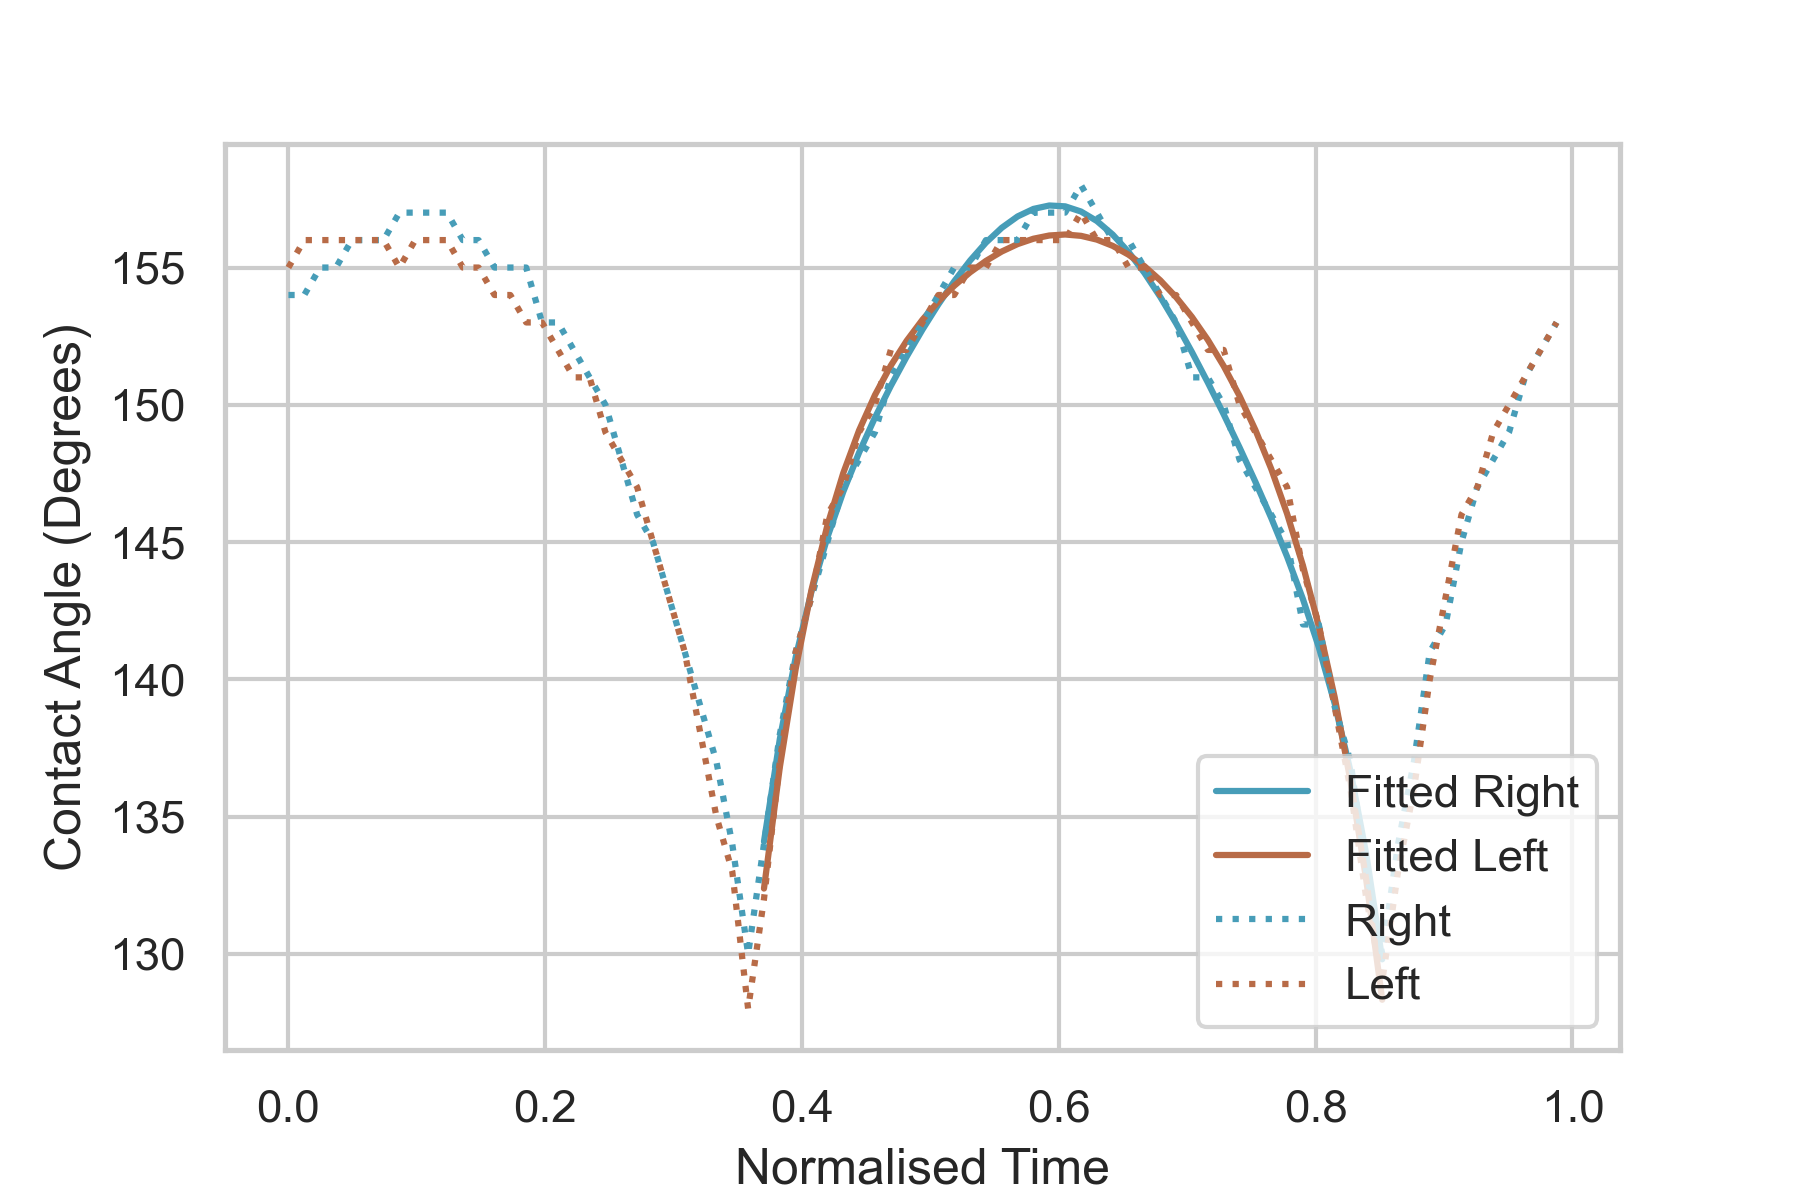
\includegraphics[width=0.5\textwidth]{Sections/Figures/B5055.png}
  \caption{B-50-5.5 slide hysteresis experiment showing Polynomial fitting}\label{Hyster}
\end{figure}
\subsection{Statistical Analysis Methodology}
The coefficient of determination ($R^2$) measured the fraction of the total variation in Y that is captured by the model. $R^2$ values were calculated to provide a quantitative measure of the polynomial's fit to the hysteresis data. In addition, the mean and standard deviation (SD) of static and advancing CA's were reported for each formulation. Comparison of the means amongst formulations were performed by one-way analysis of variance (ANOVA). ANOVA was used to evaluate whether there was any statistical evidence that the means of the sets of data differ using the F-distribution; therefore, the null hypothesis for this test was that all means were equal ($H_0: \mu_A = \mu_B =...$ ). During ANOVA, F-testing was conducted to test the underlying assumption of homoscedasticity as a preliminary step. If F > F crit  the null hypothesis was rejected and at least one of the means is statistically different'. This 'omnibus' testing (assuming a significant result) was followed up by multiple pair-wise category t-tests. The p-value was calculated to ascertain if there was a significant difference between specific individual groups. Statistical analysis between groups was primarily carried out on $\theta_A$ values as to not involve the uncertainty that is inherent from a metastable static droplet . 
\par Non-paired, two-sample unequal/equal variance (depending on the result of an initial F-test) t-testing was then performed between slides within the \emph{same} formulation to investigate the reproducibility of the dip-coating method. Factors that could affect these results include dipping speed, withdrawal speed, dipping angle etc. 
\par The null hypothesis here was that the two population’s of contact angles were the same ($H_0:\mu_1 = \mu_2$). The Alternative $H_1$ was that they were different due to non-reproducibility of the dip coating method. The inherent bias of slide selection was mitigated in-lab by choosing random slides for analysis. If the p-value was found to be above the significance level $\alpha = 0.05$, the null hypothesis was not rejected and there was not sufficient evidence to conclude non-reproducibility via dip-coating and the variance of angles that were measured in data occurred by chance or some other factor.
\subsection{Durability Testing Methodology}
'DVS Advantage' was used for \textbf{DVS testing} to determine the hygroscopicity of the coatings. 50mg of the optimised formulation samples were used due to their hydrophobic nature. A step change from 0\% RH to 90\% RH was used and ran for 750 mins to determine percentage change in mass. 
\par During \textbf{immersion testing} 2 slides of each formulation were placed into DI water in separate beakers. At 10 minute intervals up to 1 hour, the slides were taken out, dried with compressed nitrogen and static WCA recorded in triplicate. 

\begin{wrapfigure}{l}{0.17\textwidth}
\centering
    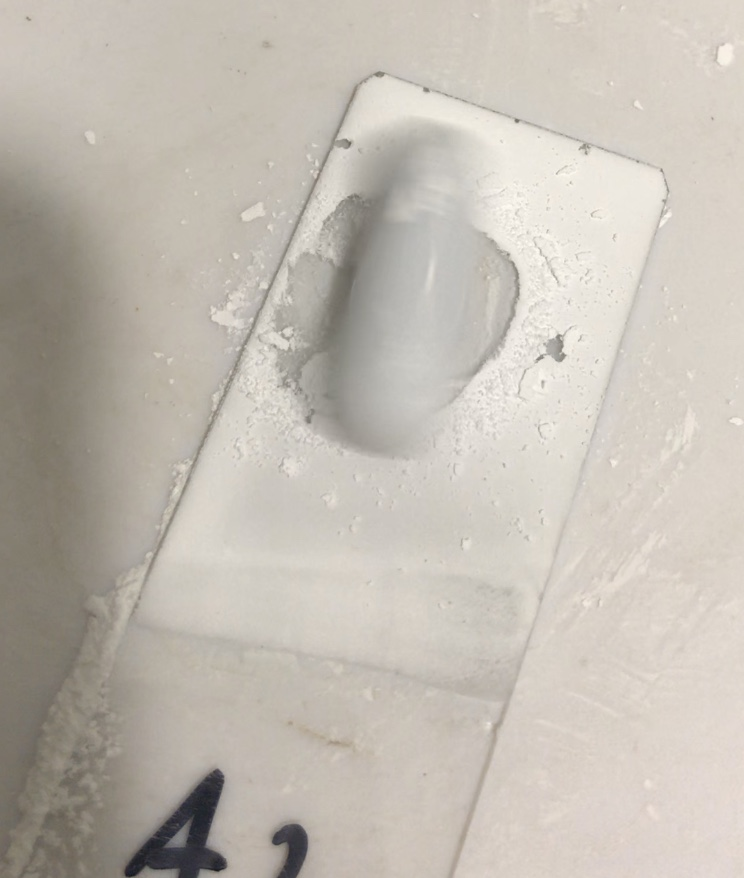
\includegraphics[width=0.1\textwidth]{Sections/Figures/MechanicalSetup.jpg}
\centering
  \caption{Stirrer causing surface mechanical abrasion}
  \label{abrasion_method}
\end{wrapfigure}

\par The qualitative \textbf{mechanical abrasion method} tested physical robustness of prepared coatings on the glass substrate. The rotation speed of a 2cm stirrer bead was kept constant at 150rpm and the time for glass to be first seen recorded, as in Figure \ref{abrasion_method}. This was repeated for 2 slides and the average determined. A 'Veho  VMS-004 microscope camera' capable of 20-400x magnification was used to take images of the area of abrasion.
\par The \textbf{outdoor test} aimed to investigate the change in film characteristics due to rain droplets and higher RH than indoors (\cite{syafiq_vengadaesvaran_ahmed_rahim_pandey_bushroa_ramesh_ramesh_2020}). 2 slides of each formulation had their static WCA measured before being placed outside on the window sill in SW7. Temperature and RH were monitored from BBC Weather for 5 days and the static WCA measured after being blown dry with compressed N$_2$. 





\section{Results \& Discussion}

\subsection{Static WCA and Observations}
\begin{figure}[h!]
\centering
  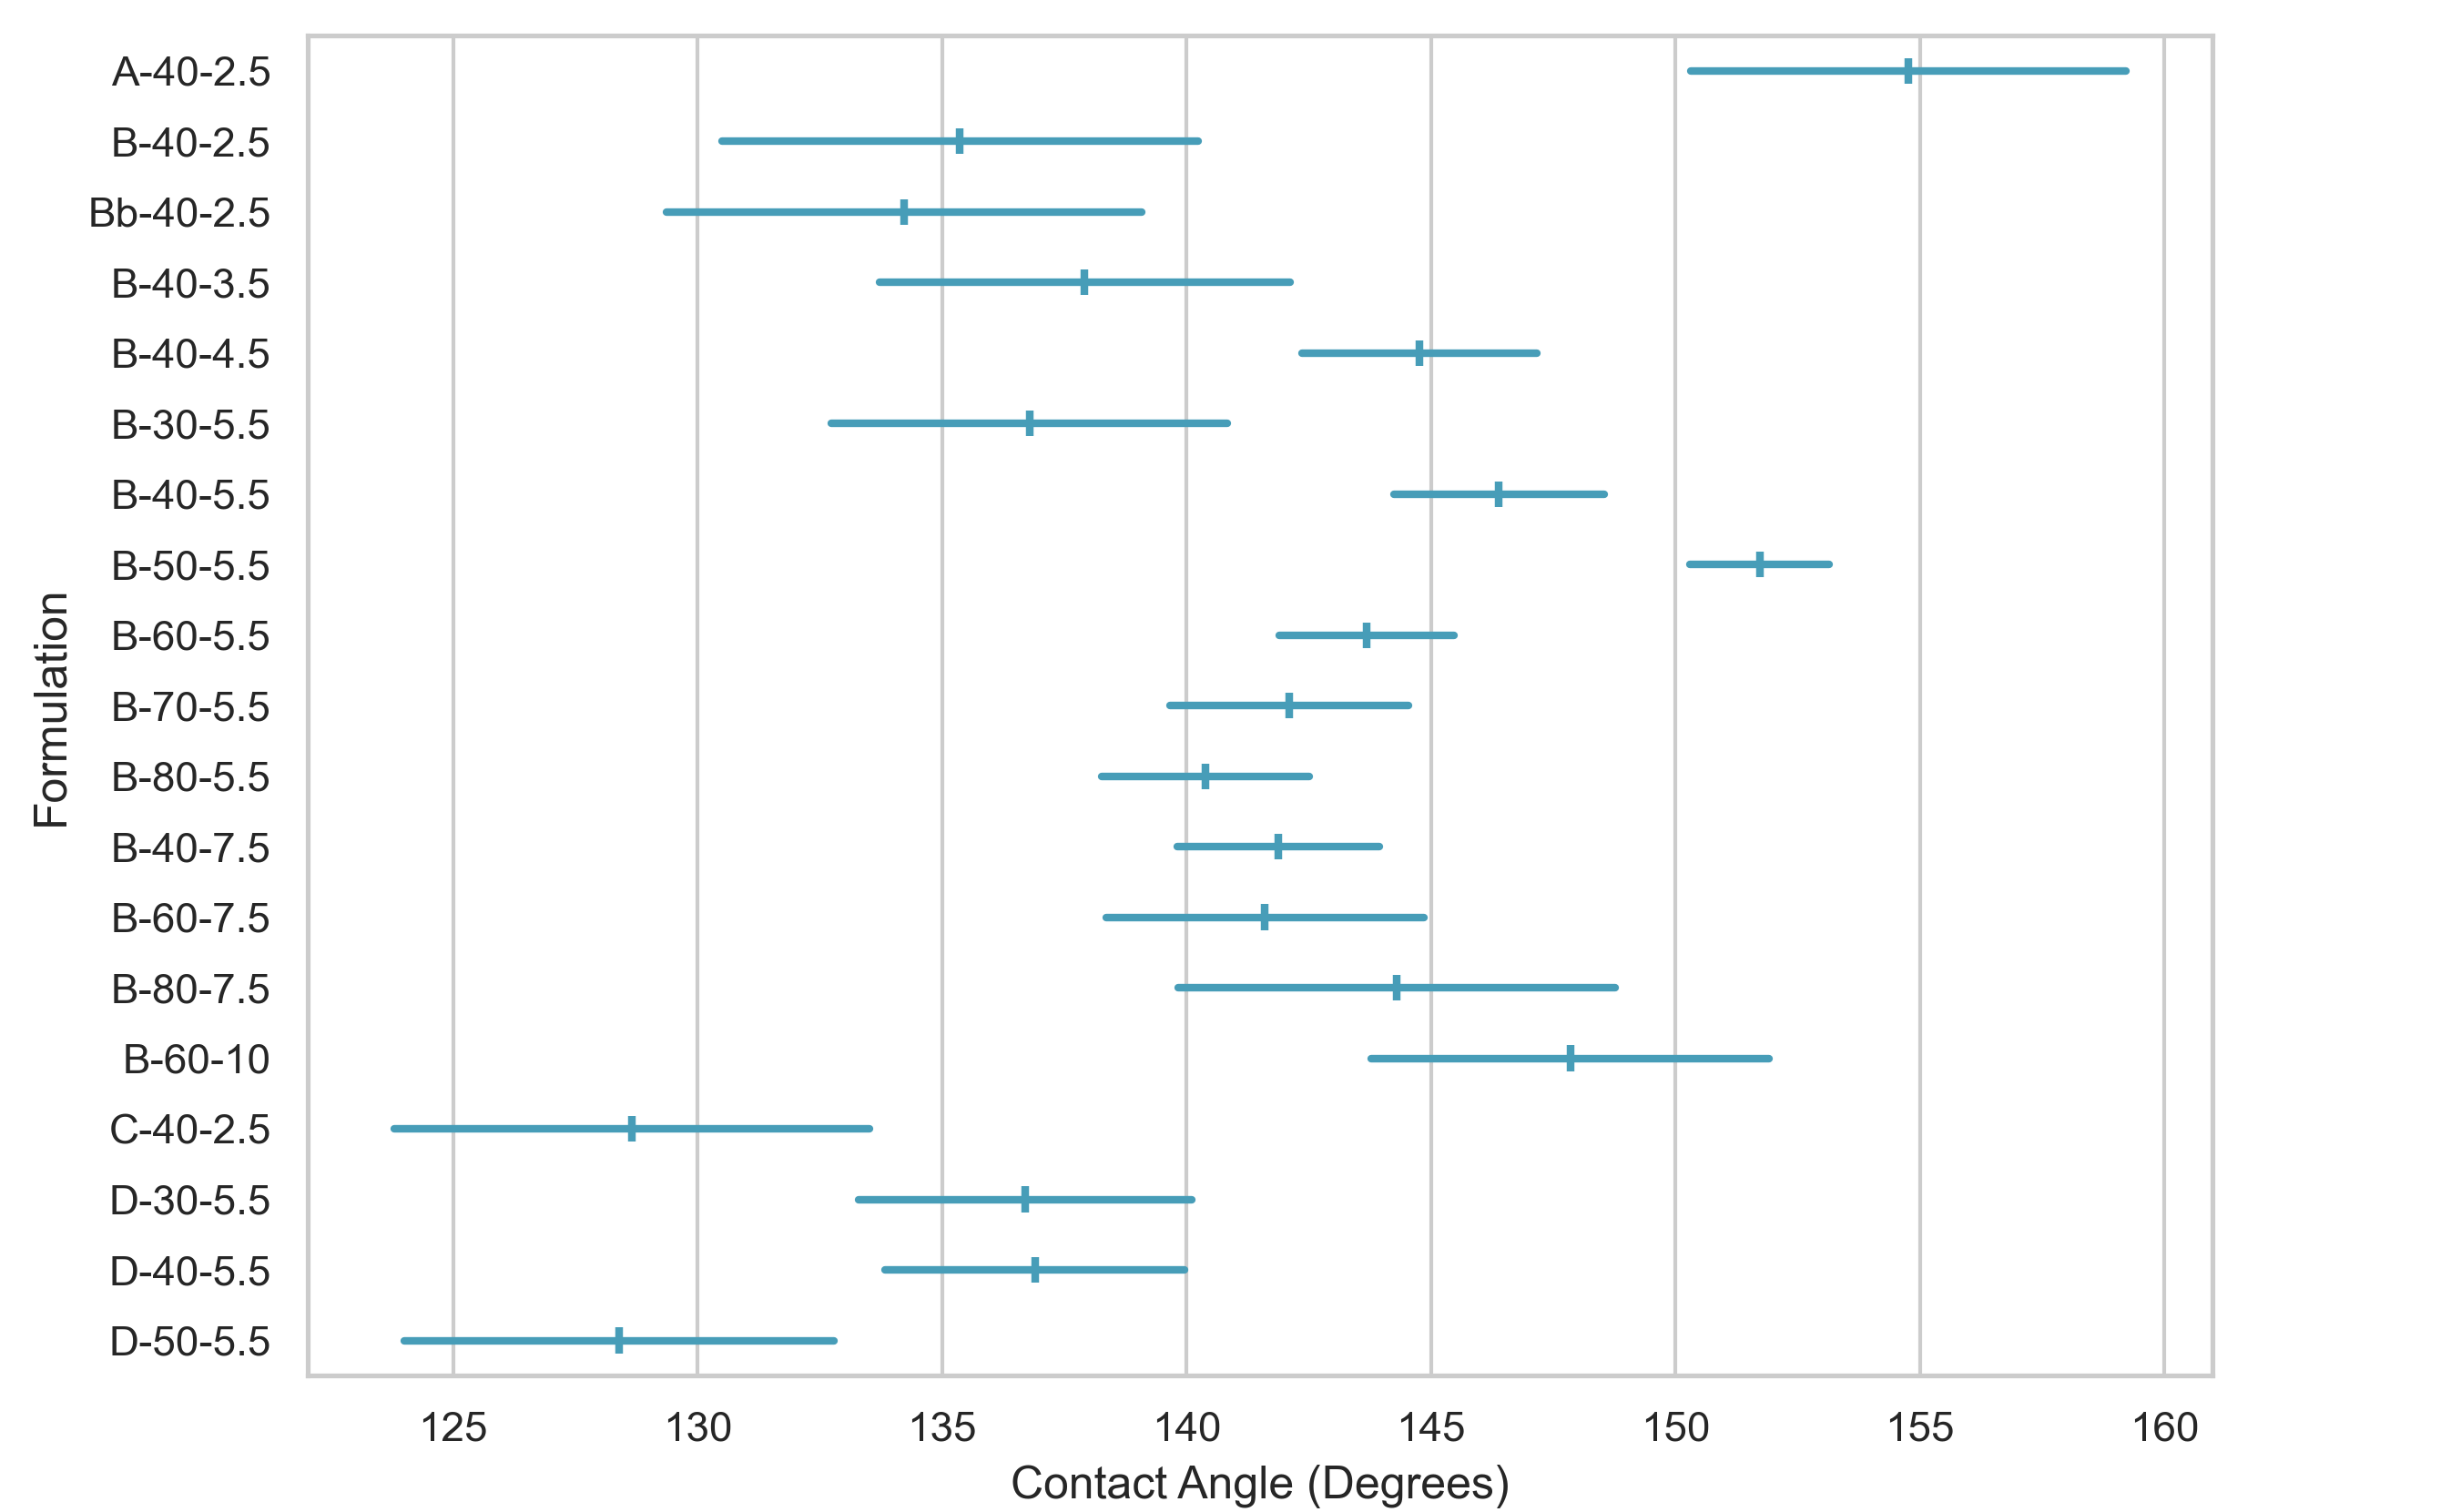
\includegraphics[width=0.523\textwidth]{Sections/Figures/StaticBlue2.png}
  \caption{Static WCA plot for produced formulations presenting mean  \& standard deviation. Films that exhibited absorption are omitted.}\label{CAs}
\end{figure} 

\begin{wrapfigure}{r}{0.2\textwidth}
\centering
    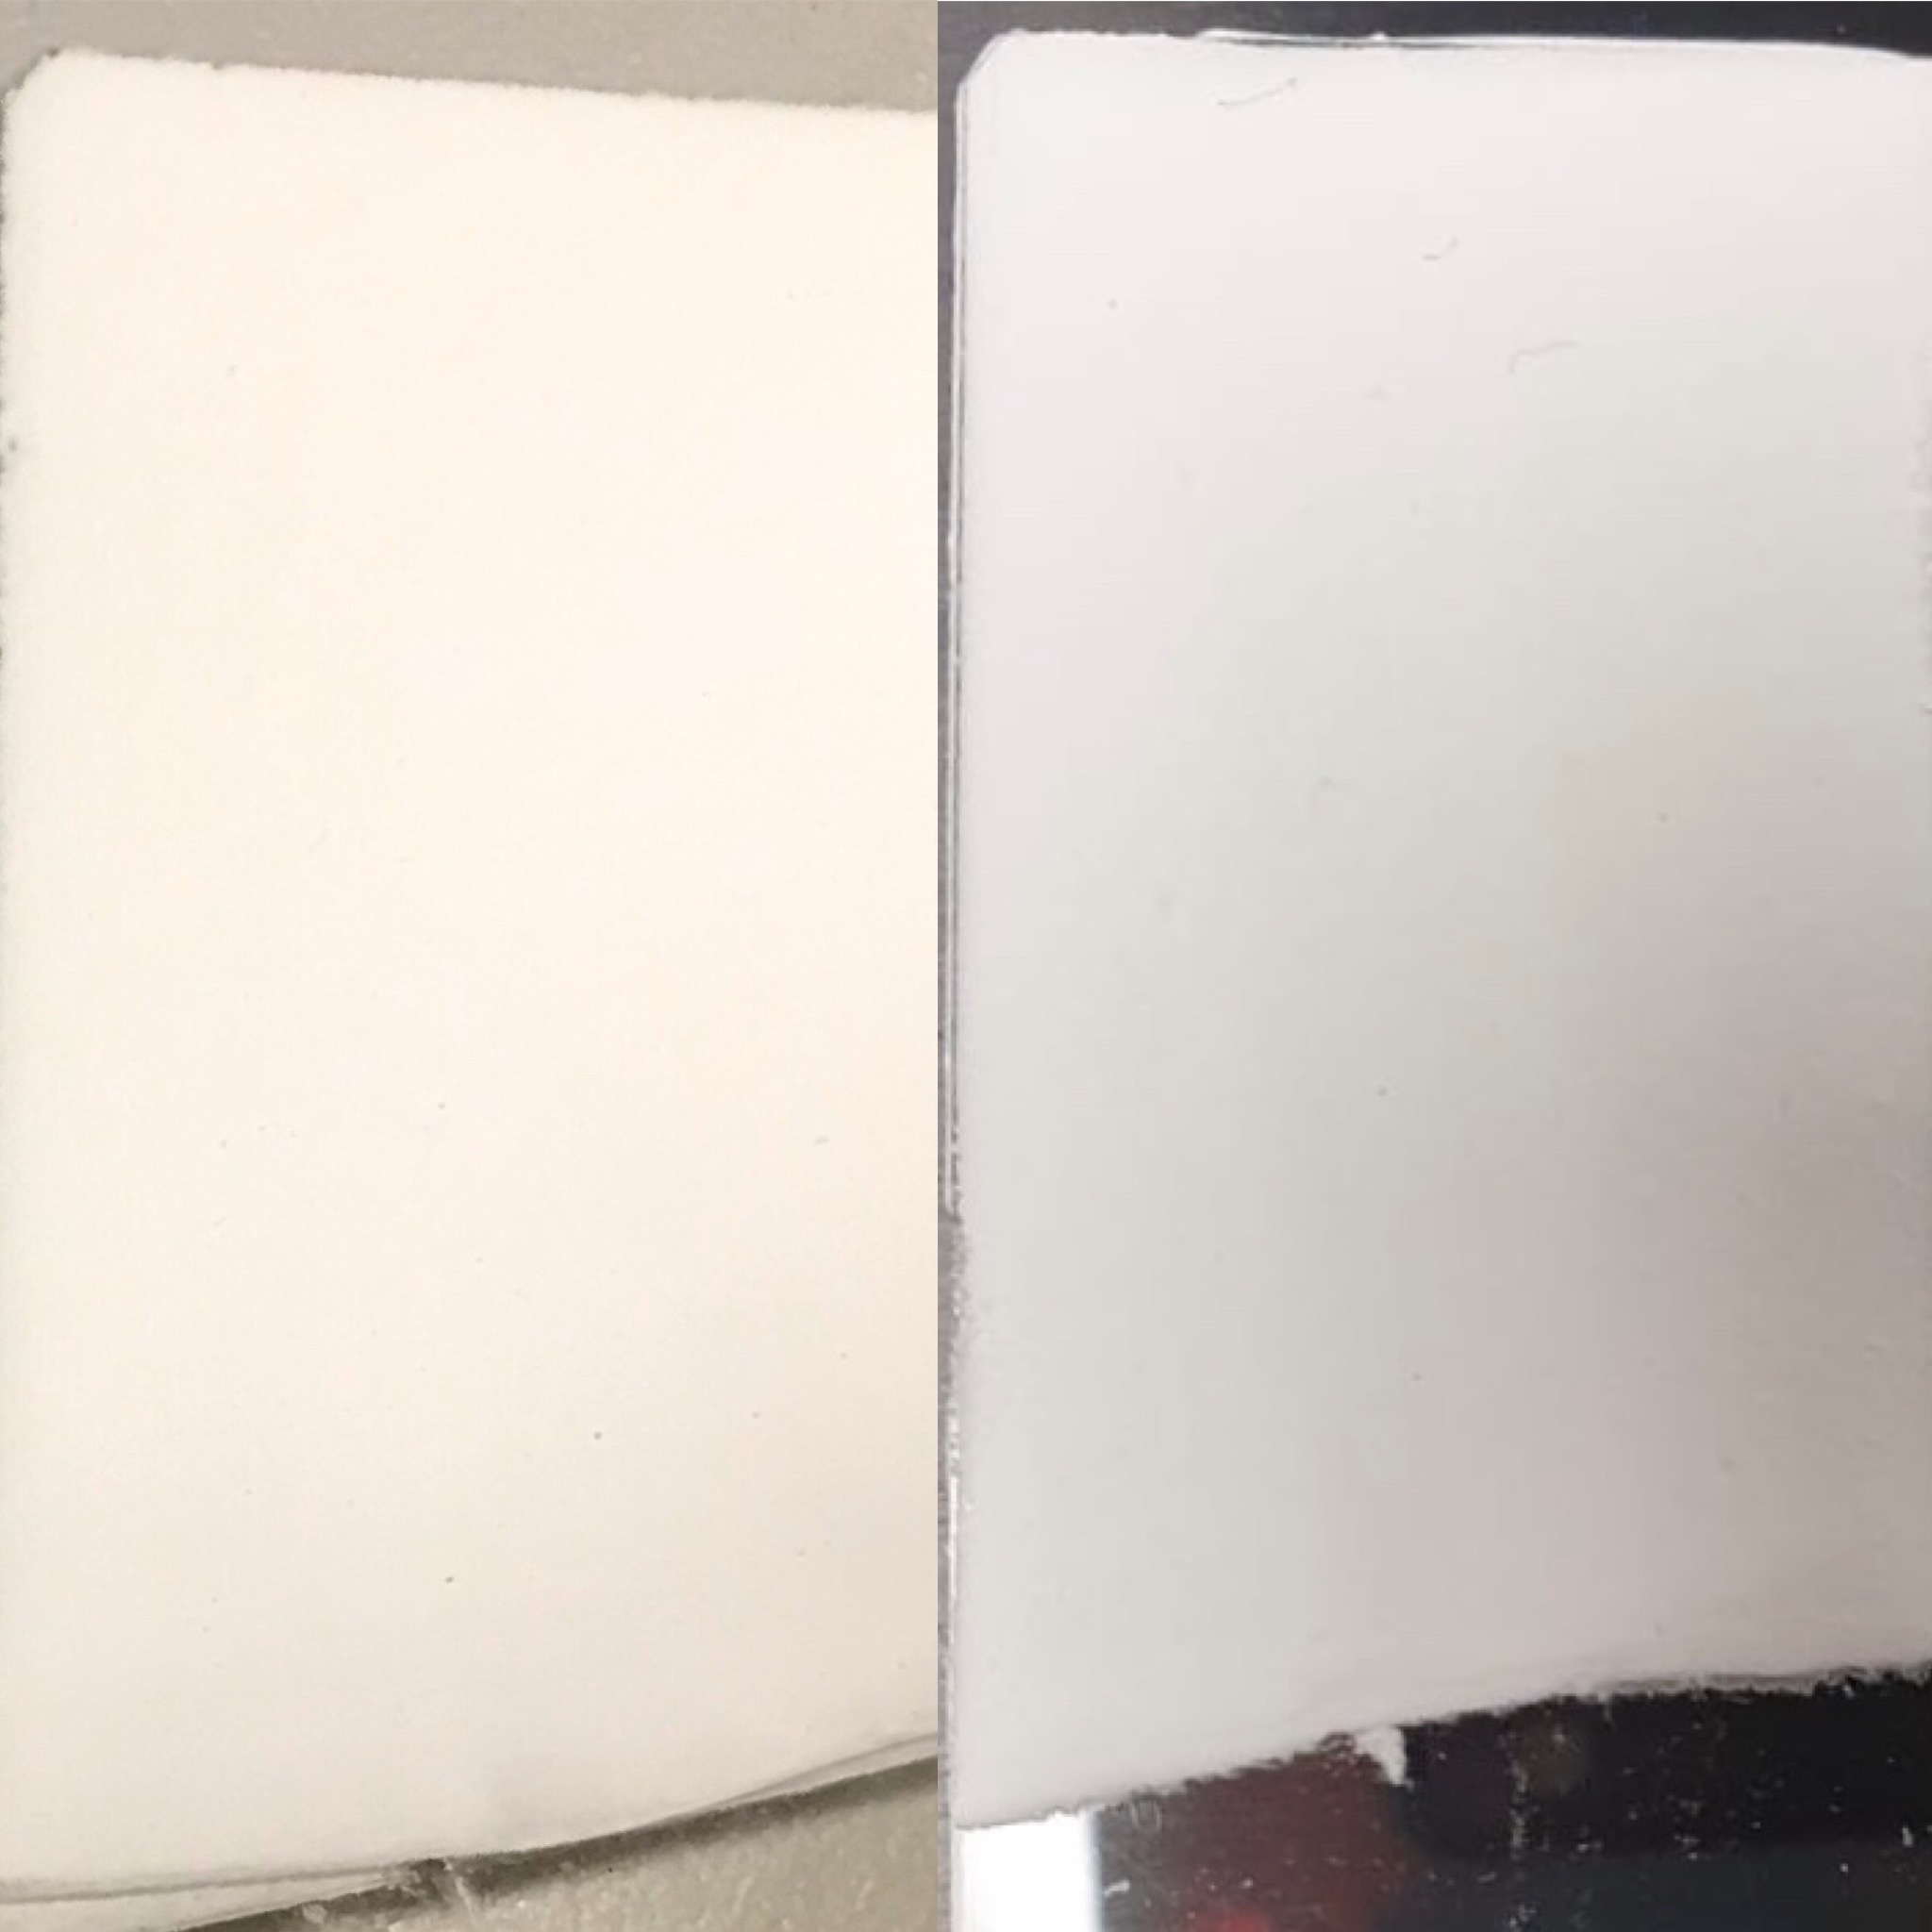
\includegraphics[width=0.1\textwidth]{Sections/Figures/AandB.jpeg}

  \caption{Side by side comparison of A-40-2.5(left) B-50-5.5(right)}
  \label{Comp}
\end{wrapfigure}

Figure \ref{CAs} presents a global view of collected static WCA's; from here it can be concluded that B-50-5.5 is the optimal formulation being statistically higher than all other starch based formulations (bar B-60-10 which exhibited in-homogeneous, powdery and unacceptable film properties). B-50-5.5 overlapped with A-40-2.5, showing comparable static water contact angles.

\begin{wrapfigure}{r}{0.2\textwidth}
\centering
    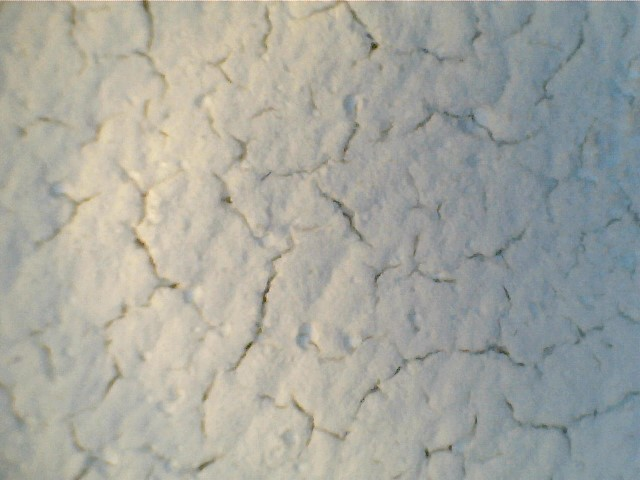
\includegraphics[width=0.1\textwidth]{Sections/Figures/WIN_20201203_13_09_29_Pro.jpg}
  \caption{Bb-40-2.5 image at 25X magnification}
  \label{Bcrack}
\end{wrapfigure}
\par \textbf{Observations} worth noting here were the failure of attempted starch modifications. It was hypothesised that OMS produced a more hydrophobic film (\cite{jiang_dai_qin_xiong_sun_2016}) but exploratory experiments yielded observations of cracking and non-continuous film formation. It is postulated that the increased hydrophobicity of the particles interfered with the gelatinisation process of starch and therefore prohibited optimal dispersion of the OMS in 1:1 DI Water to Ethanol mixture. OMS was not able to be characterised as droplets were absorbed into the surface. TEOS films on the other hand showed improved film forming ability. However, TEOS and the other starch-inorganic hybrid nano-silica (Formulation C), exhibited sub-par hydrophobicity. It is possible that these inorganic silica particles, whether formed from TEOS (\cite{TEOS}) in D or from silica nanoparticles in C interfered with the binding action of starch. 'Bb-40-2.5' was investigated to determine influence of drying rate on WCA. As seen in figure \ref{CAs} there was a 1.5° reduction in static CA compared to the vacuum cupboard dried B-40-2.5 and crack formation was observed due to the increased drying rate as in Figure \ref{Bcrack}.


\subsection{Optimisation of Formulation B}
\begin{figure}[h!]
\centering
  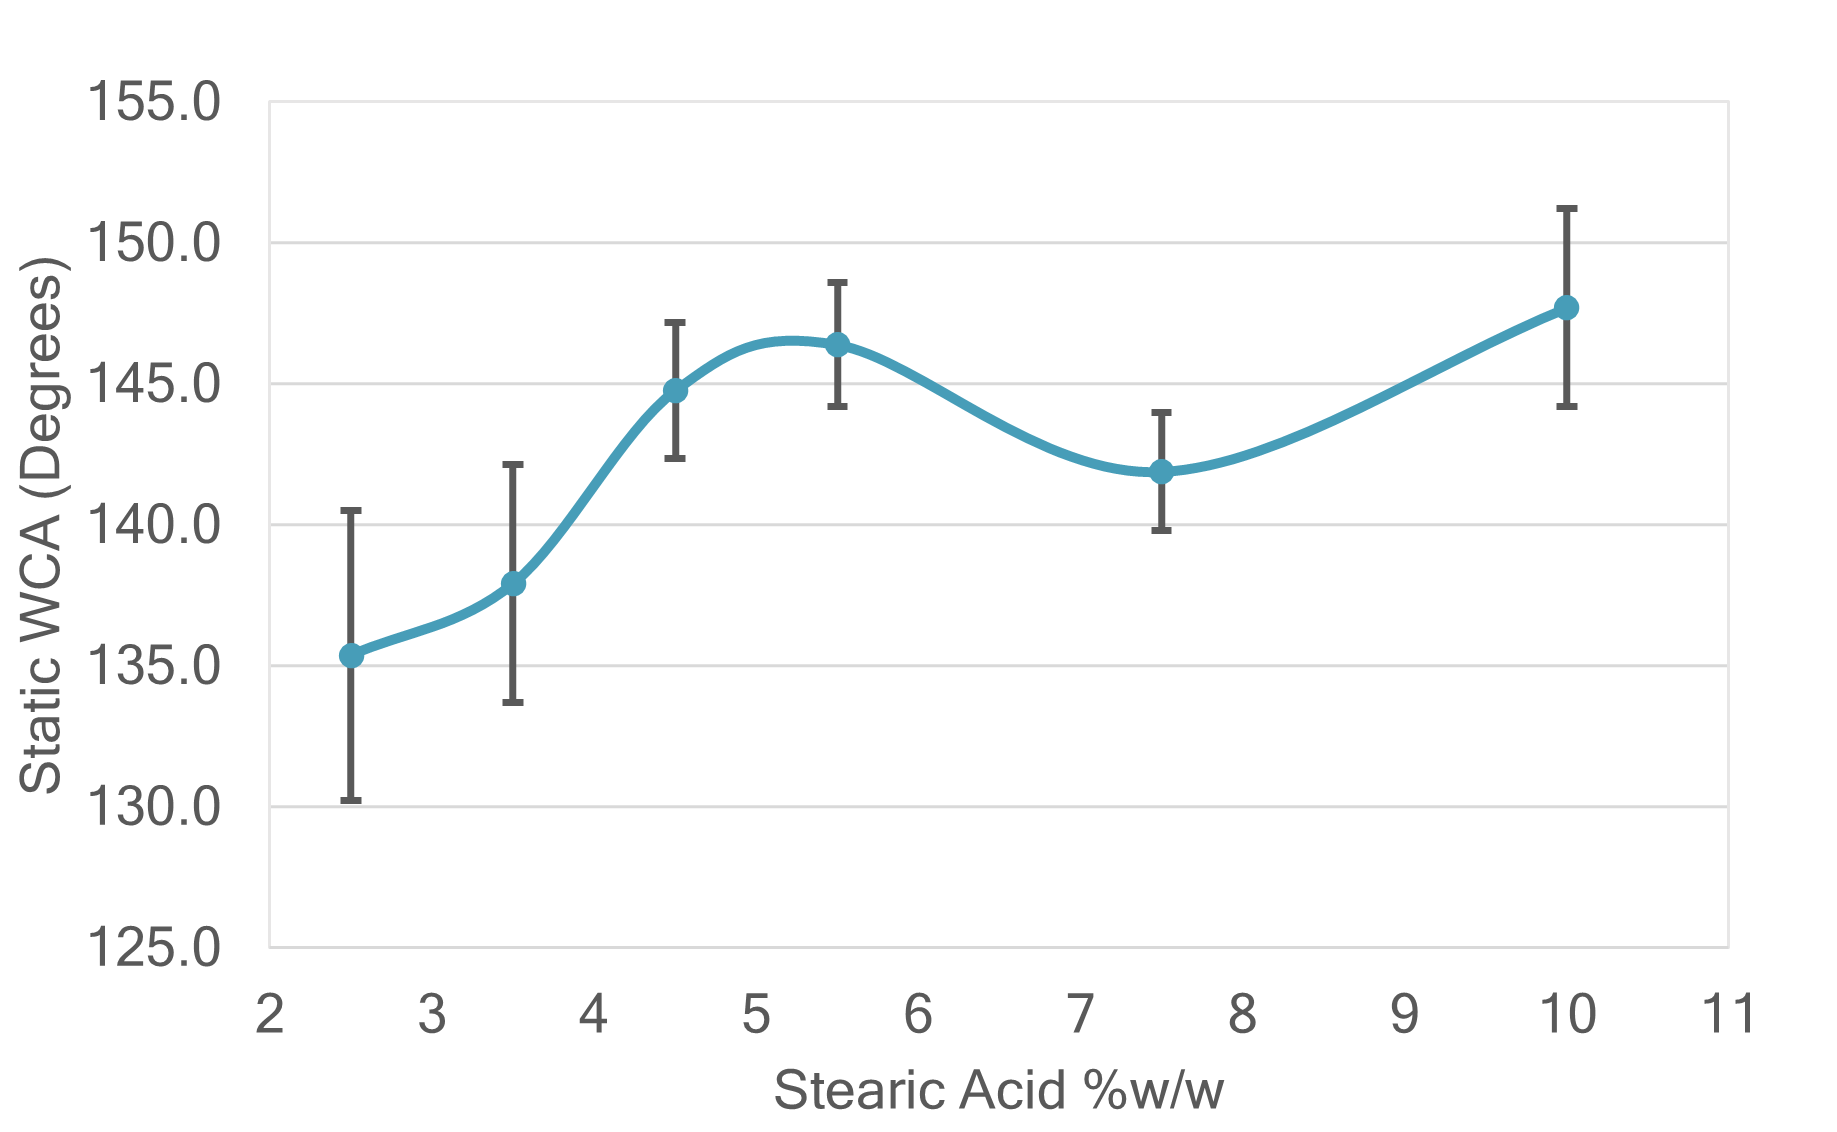
\includegraphics[width=0.4\textwidth]{Sections/Figures/SAOptimise.png}
  \caption{The effect of increasing stearic acid \%w/w for 40\% w/w hydrophobic powder of formulation B}\label{SAOpt}
\end{figure}

As hydrophobic stearic acid (SA) \%w/w was increased, a local maximum was observed; figure \ref{SAOpt} shows that for 40\% w/w SHP, the optimum stearic acid addition content in calcium carbonate was 5.5 \% w/w with a water CA of 146.4° $\pm$ 2.2°. Beyond the optimum, the film became excessively powdery due to physisorbed SA SHP on the calcite surface resulting in a fluctuating WCA with a high SD. Therefore, the optimum was determined at 5.5\%w/w to align with the objective of producing a homogeneous and continuous film. Pure stearic acid has a CA of ~ 120° so it is expected that further increase in SA content will lead to a drop in CA.

\begin{figure}[h!]
\centering
  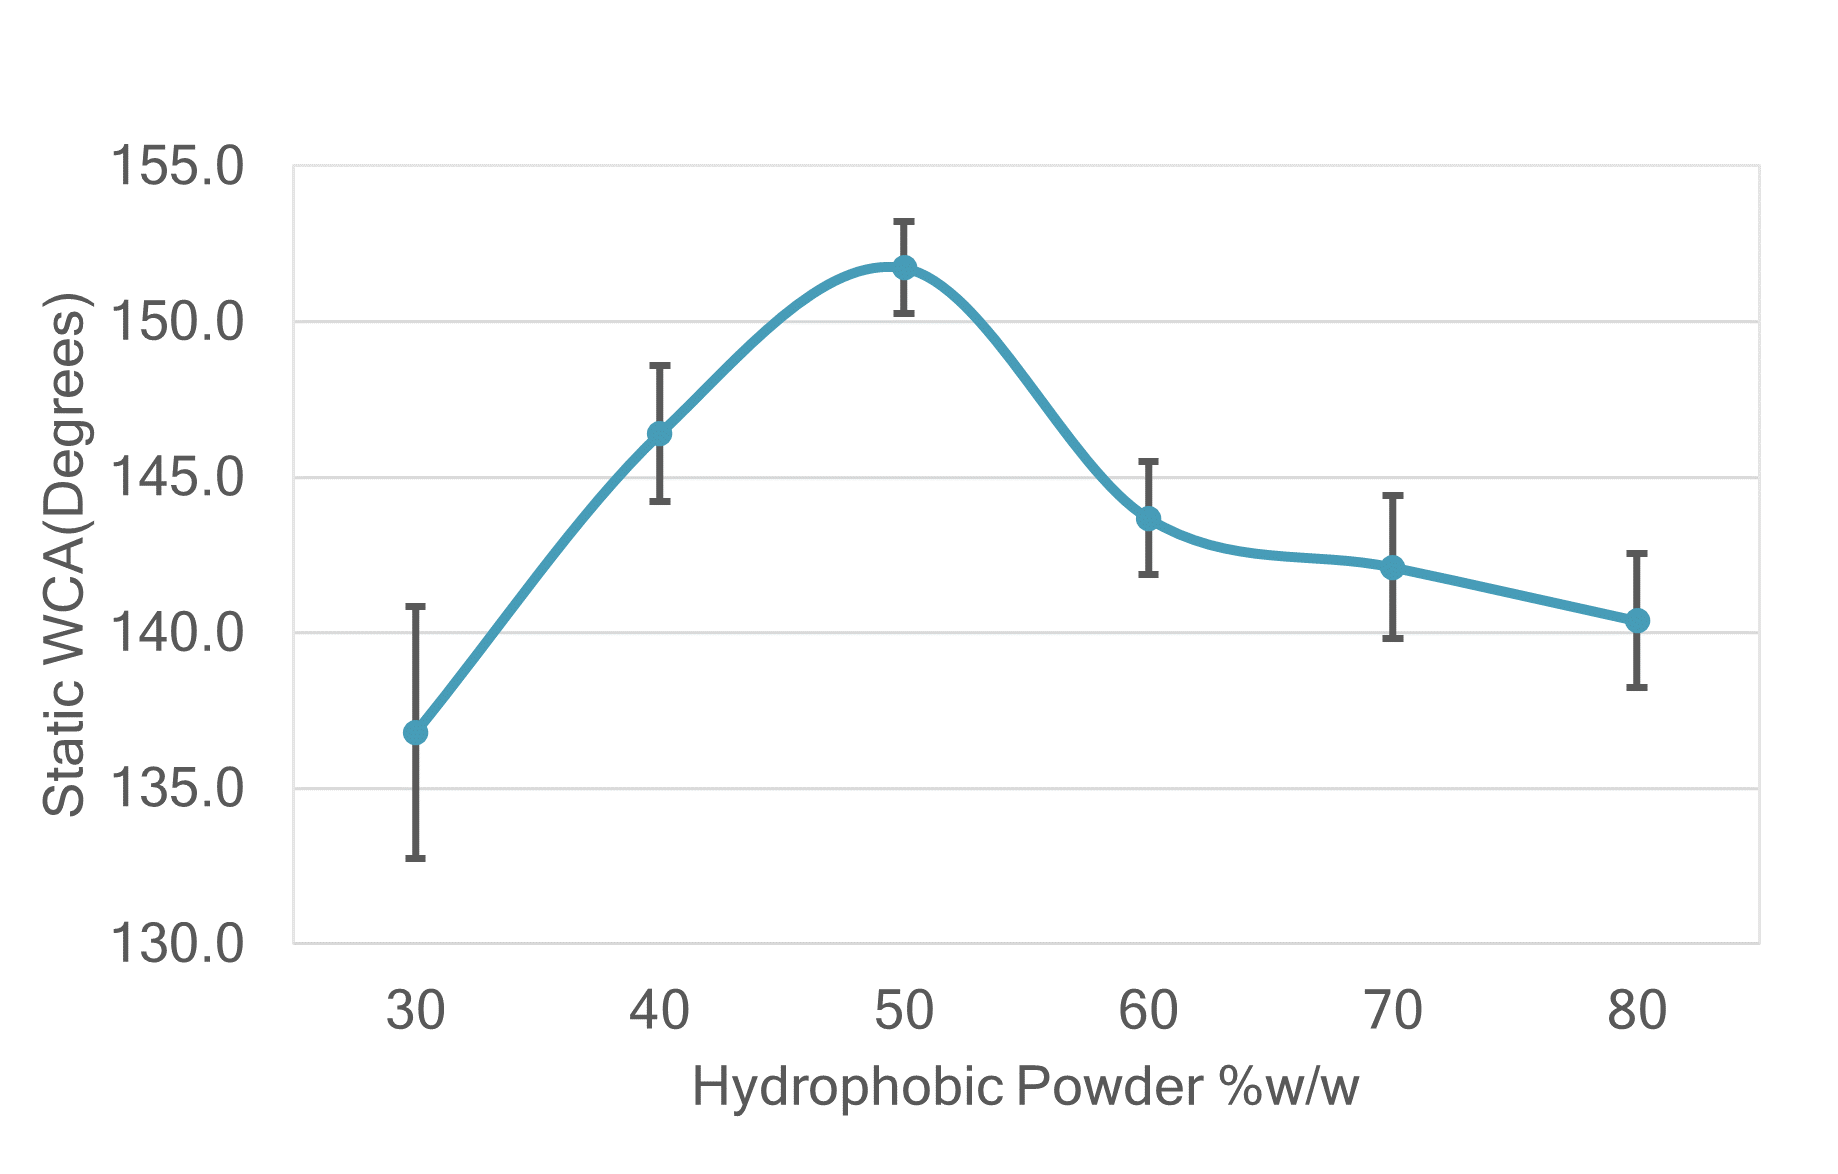
\includegraphics[width=0.4\textwidth]{Sections/Figures/HPOptimise.png}
  \caption{The effect of increasing hydrophobic powder content for 5.5\%w/w stearic acid of formulation B }\label{HPOpt}
\end{figure}

Figure \ref{HPOpt} shows that for a SA weight \% of 5.5, the optimum addition of SHP was 50\%w/w with a WCA of 151.7 $^\circ$ $\pm$ 1.5. Increasing SHP content improved hydrophobicity and viscosity for adhesion during dip coating. However, there was a compromise; as the binding solvent became more saturated there was a corresponding increase in in-homogenous film formation which featured pockets of non-bound powder. An optimum was therefore chosen to avoid this.   


\subsection{Receding Contact Angle}
Measuring $\theta_R$ using the sessile drop method led to considerable difficulty due to the rough surface topography of the samples. The droplet did not recede when water was withdrawn via the needle as the contact line remained pinned. This was ascribed to the local defect mechanism (\cite{hong_chang_chou_chan_sheng_tsao_2011}); the presence of local defects that were considerably more wettable than the rest of the surface. Instead of receding, the withdrawal of the water caused a change of the droplet shape from a spherical cap to a conical one as demonstrated by figure \ref{Cone}. This effect was enhanced through the adhesion of water to the hydrophilic steel needle.   
\par When even more water was withdrawn, the water snapped away from the needle. This indicated that the adhesion between the water and the films being analysed was higher than the cohesion between water molecules. Due to these reasons, $\theta_R$ could not be measured on any of our samples using this method. 



\begin{figure}[h!]
\centering
  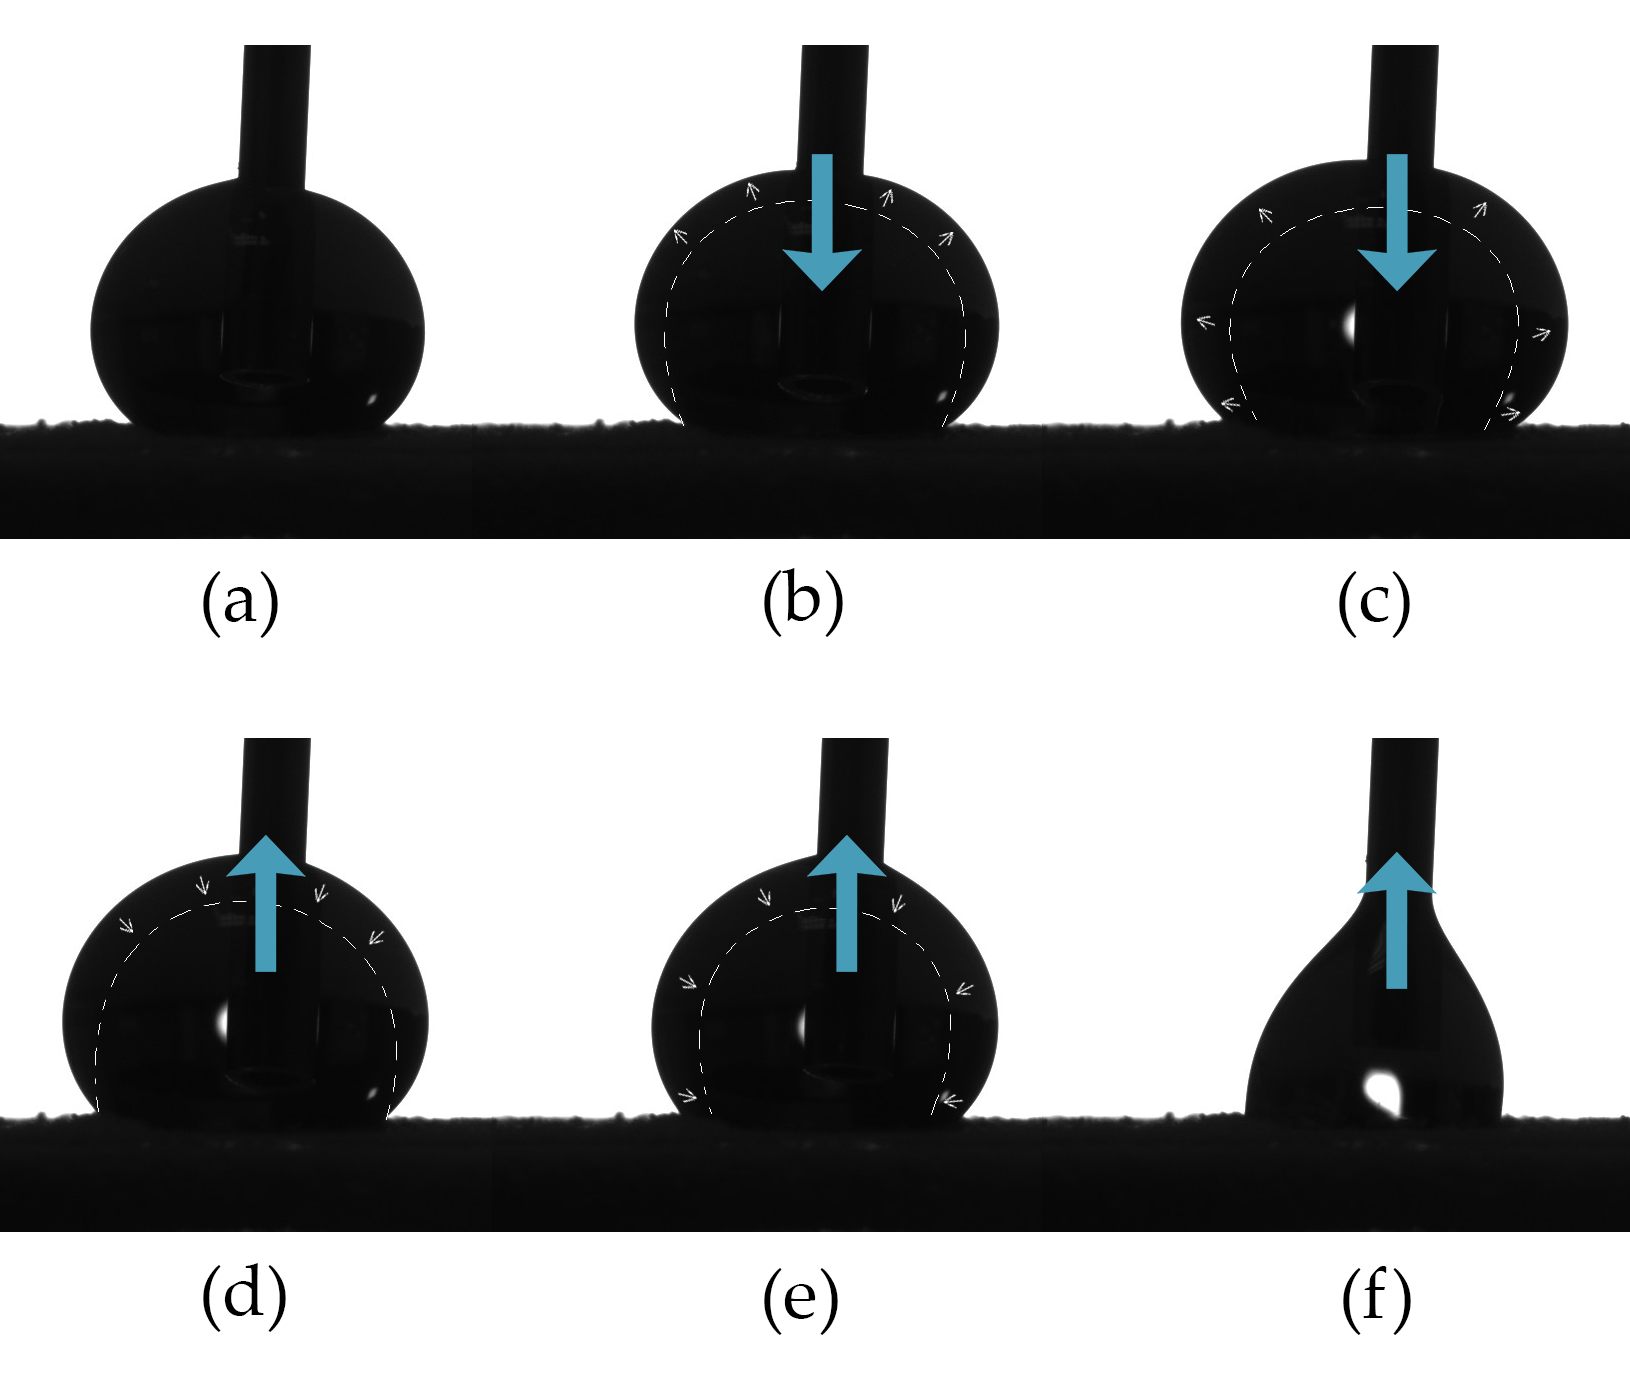
\includegraphics[width=0.45\textwidth]{Sections/Figures/sessile3.png}
  \caption{Photograph sequence showing the sessile-droplet method with receding contact line pinning on a formulation C slide\footnotemark: (a) The initial droplet volume ($20\mu L$); (b) Volume dispense increment before contact line advancement; (c) contact-line advancement due to volume increments dispensed into droplet; (d) reduction in droplet volume before droplet starts receding (with a pinned contact line); (e) A suction increment showing a receding contact line; (f) Further reduction in volume with a pinned contact line on slide surface showing the conical-esque shape.}\label{Cone}
\end{figure} 
\footnotetext{Formulation C was chosen for figure 2 as the transition to a conical shape was more apparent and extreme on this film}
\newpage
\subsection{Statistical Analysis of $\theta_A$}
%Contact Angle Measurements}
\begin{figure}[h!]
\centering
  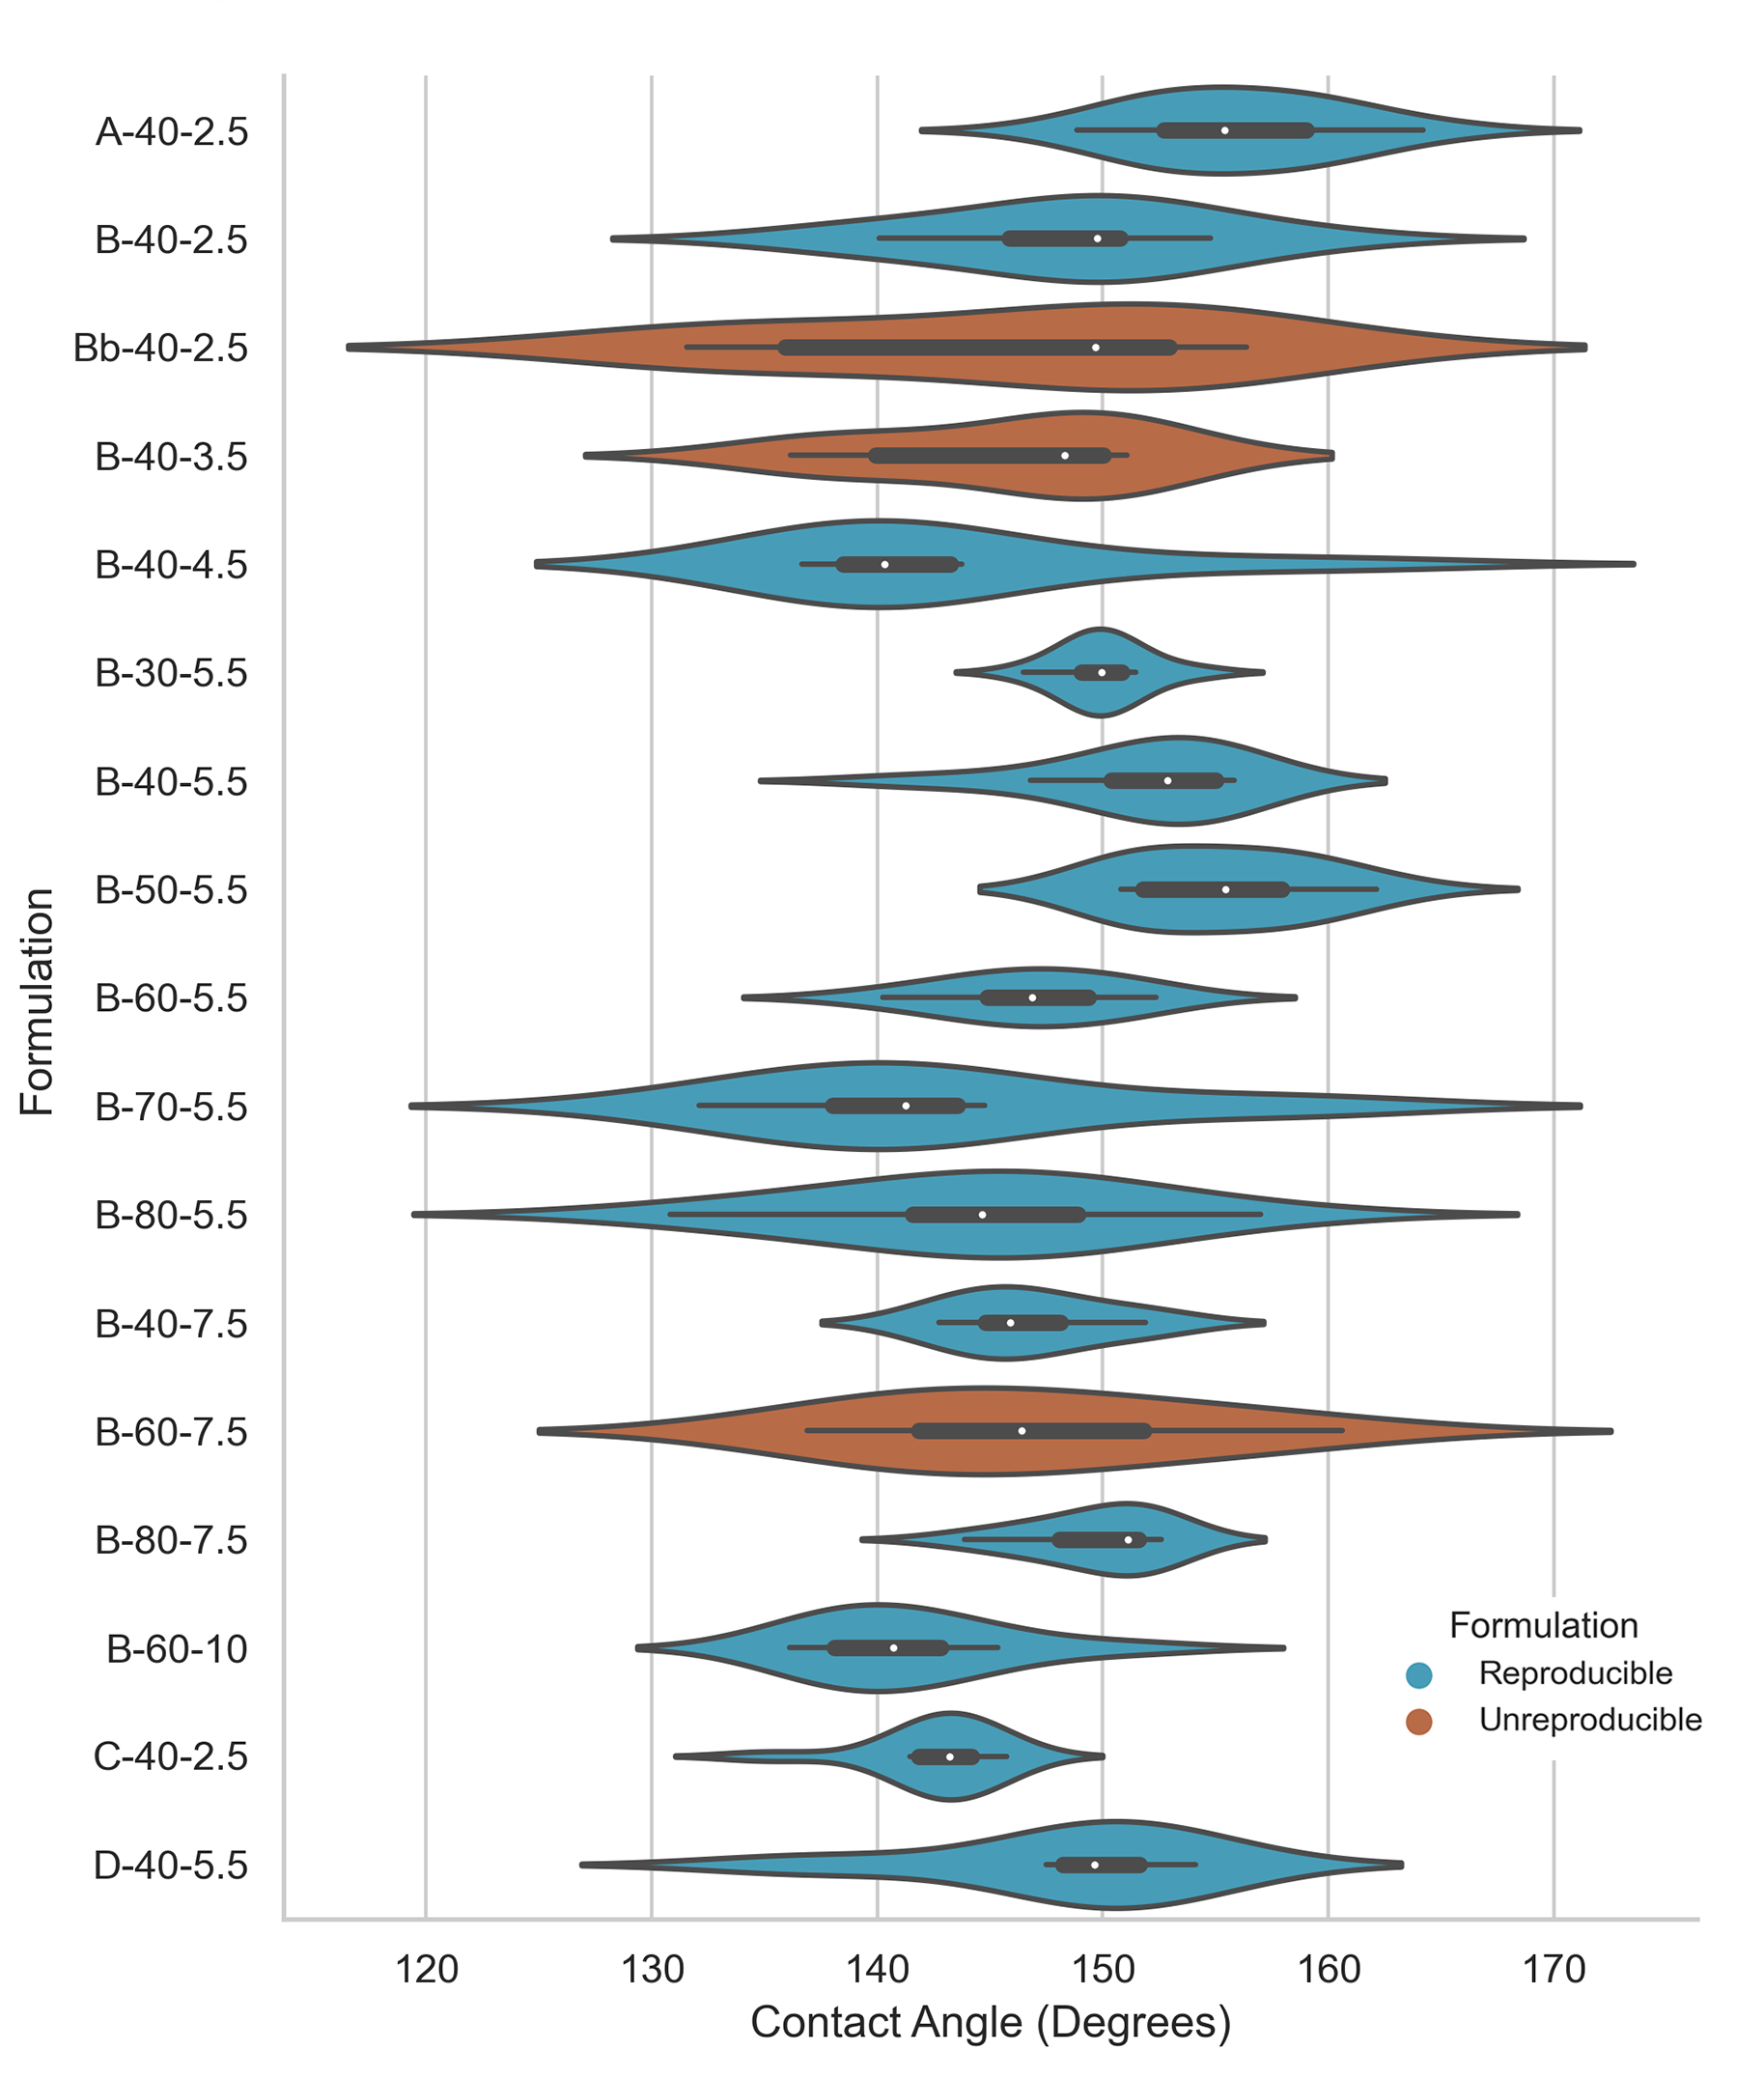
\includegraphics[width=0.5\textwidth]{Sections/Figures/tiny.png}
  \caption{Violin plot of $\theta_A$ for each formulation alongside box and whisker plots. Violin shape is a  kernel density estimation of the underlying $\theta_A$ distribution.}\label{CA}
\end{figure} 

Figure \ref{CA} depicts the advancing contact angle measurements, which were all achieved with well fitting polynomials with a mean $R^2$ value of 0.99 from all experiments, indicating excellent goodness-of-fit. 
\par During intra-formulation slide-to-slide analysis of $\theta_A$, a P value of $x$ can be understood as an $x\%$ likelihood that the difference in means was due to random chance. Conventionally, a P value < $\alpha = 0.05$ is significant in which case we rejected the null hypothesis, $H_0:\mu_1 = \mu_2$.  If the P value was greater than 0.05, we do not reject the null hypothesis and concluded no statistical significant difference between the two slides. 
\par The only formulations that exhibited statistically significant differences between slides within the 95\% confidence interval were Bb-40-2.5, B-40-3.5 \& B-60-7.5 as shown in Figure \ref{CA} as 'unreproducible'. For the remaining formulations, it can be assumed that dip coating played an insignificant role in variance. Data can be safely grouped together and analysed as the remaining possible causes of formulation variance are chance and surface in-homogeneity. The interquartile range (IQR) for each formulations is presented in figure \ref{CA} and is an indicator of surface homogeneity for each film, with outliers accounted for. It was concluded that all reproducible films showed comparable surface homogeneity, attesting to the viability of a starch superhydrophobic films.
\par The null hypothesis \emph{between} the starch-based film formulations was that of identical means ($H_0: \mu_A = \mu_B = \mu_C =...$). ANOVA was carried out on all starch-based films. With a calculated F-statistic and F crit of $4.560159>1.699042$ respectively, the null hypothesis was rejected and it was concluded that at least one of the formulations exhibited statistical difference. Since this was simply an 'omnibus' test, further t-testing was performed to investigate pair-wise statistical differences between formulations; namely B-50-5.5. B-50-5.5 was statistically different when compared to B-40-5.5 with a 95\% likelihood, and statistically different to all other formulations with at \emph{least} a 99.5\% liklihood. B-50-5.5, the optimised formulation, therefore features statistically superior $\theta_A$'s to the other starch formulations.
\par Conversely, with a p-value of $0.6695104>0.05$, the null hypothesis $H_0: \mu_B_-_5_0_-_5_._5 = \mu_A_-_4_0_-_2_._5$ could not have been rejected. The measured $\theta_A$'s for B-50-5.5 and A-40-2.5 were \emph{not} statistically different. This leads again to the conclusion that starch at 5.5\% w/w SA and 50\% w/w functionalised powder is a viable replacement for toluene and PE as presented by \cite{khoo_lim_2017}. The films exhibited comparable super hydrophobic contact angles and surface homogeneities (IQR's) as shown in figure \ref{CA}.



\subsection{Durability Characterisation}
\begin{figure}[H]
\centering
\begin{subfigure}{.22\textwidth}
%  \centering
  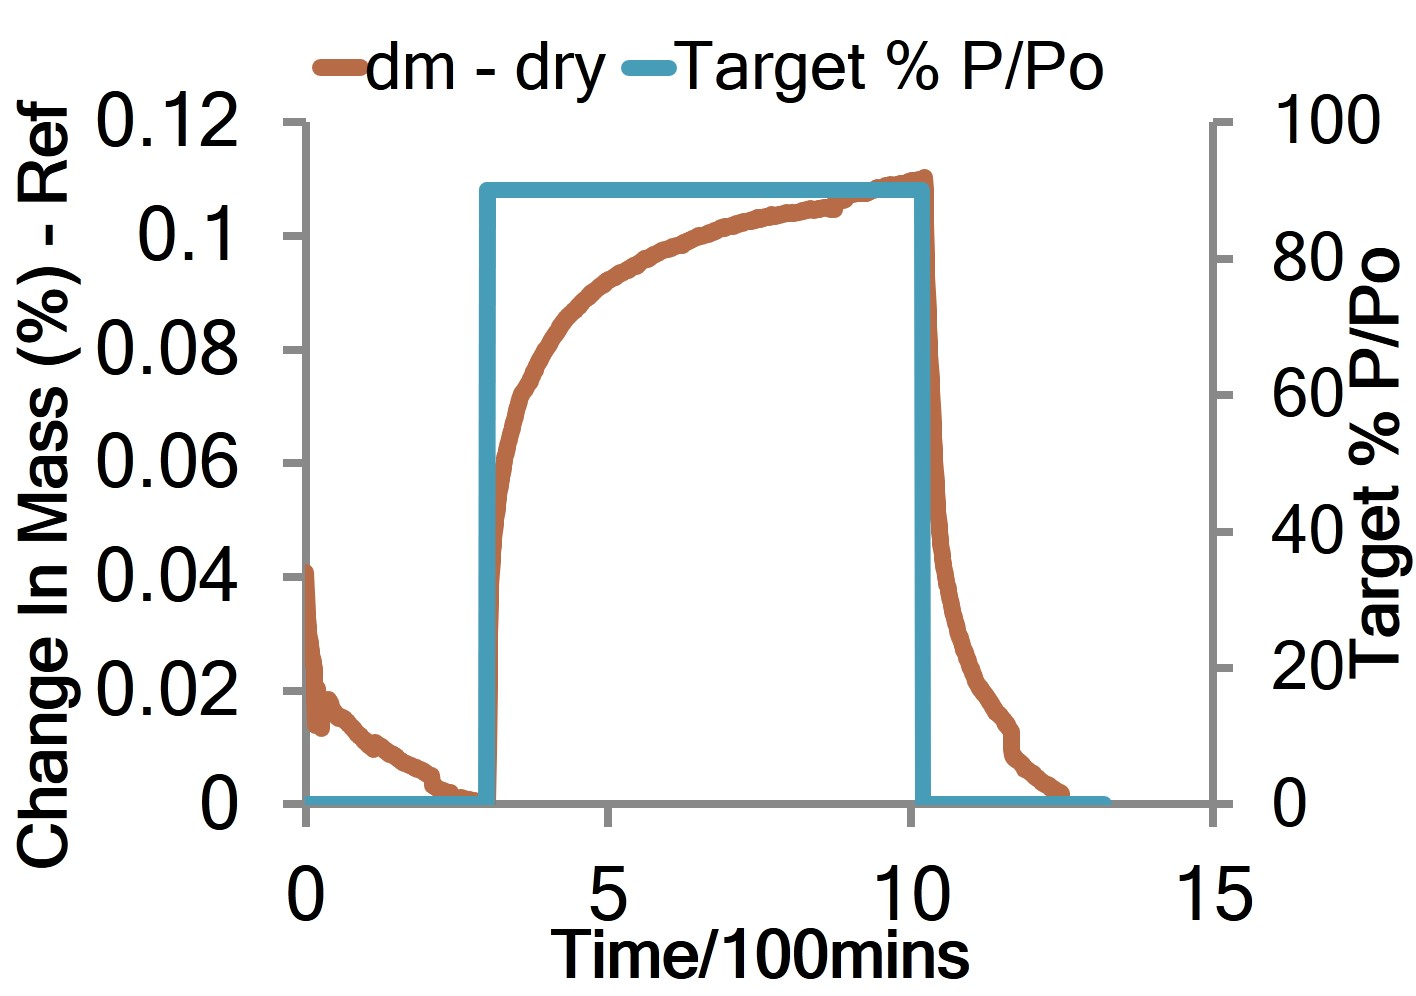
\includegraphics[width=1\linewidth]{Sections/Figures/DVSA.jpg}
  \caption{A-40-2.5}
  \label{fig:sub1}
\end{subfigure}
%.48 before
\begin{subfigure}{.22\textwidth}
%  \centering
  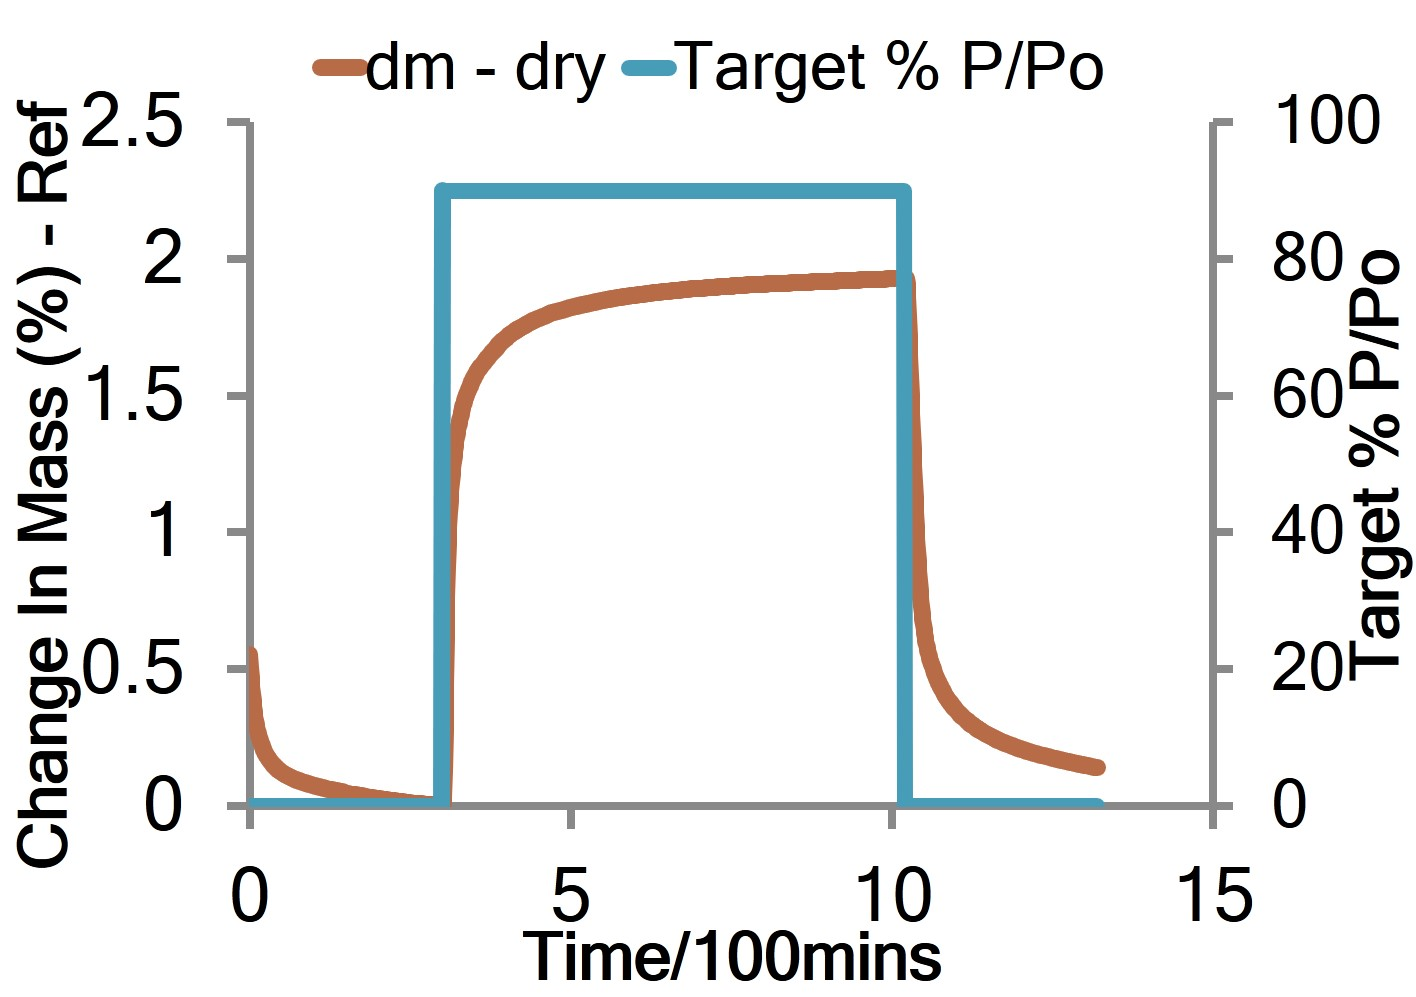
\includegraphics[width=1\linewidth]{Sections/Figures/DVSB.jpg}
  \caption{B-50-5.5}
  \label{fig:sub2}
\end{subfigure}
\caption{DVS Advance traces taken at 24.7 °C}
\label{fig:test}
\end{figure}

\textbf{DVS experiments} were completed allowing sufficient time for plateaus at 90\% RH. It has been concluded that 'B-50-5.5' is 17.5x more hygroscopic than 'A-40-2.5'. It was promising however that 'B-50-5.5' is 8x less hygroscopic than native corn starch. The higher hygroscopicity is due to the inherent hydrophilicity of the hydroxyl groups on starch polymers. Smaller step changes can be used to determine a potential type ii isotherm (\cite{starch_dvs}). 
\par \textbf{Immersion tests} studied the formulation’s hydrophobic durability while the slides were in prolonged contact with water. From visual observations, upon immersion the surface became reflective (Figure \ref{silver}) as a result of a pinned air layer, characteristic of a superhydrophobic coating in the Cassie Baxter regime, as mentioned.  When slides were removed, the surface appeared dry regardless of drying with compressed N$_2$. 

\begin{wrapfigure}{l}{0.2\textwidth}
\centering
    \includegraphics[width=0.1\textwidth]{Sections/Figures/silver.png}
  \caption{Reflection on an A-40-2.5 slide resulting from pinned air layer}
  \label{silver}
\end{wrapfigure}



%\begin{figure}[h!]
%\centering
%  \includegraphics[width=0.15\textwidth]{Sections/Figures%/silver.png}
%  \caption{Reflection on an A-40-2.5 slide resulting from %pinned air layer}\label{silver}
%\end{figure}




\begin{figure}[h!]
\centering
  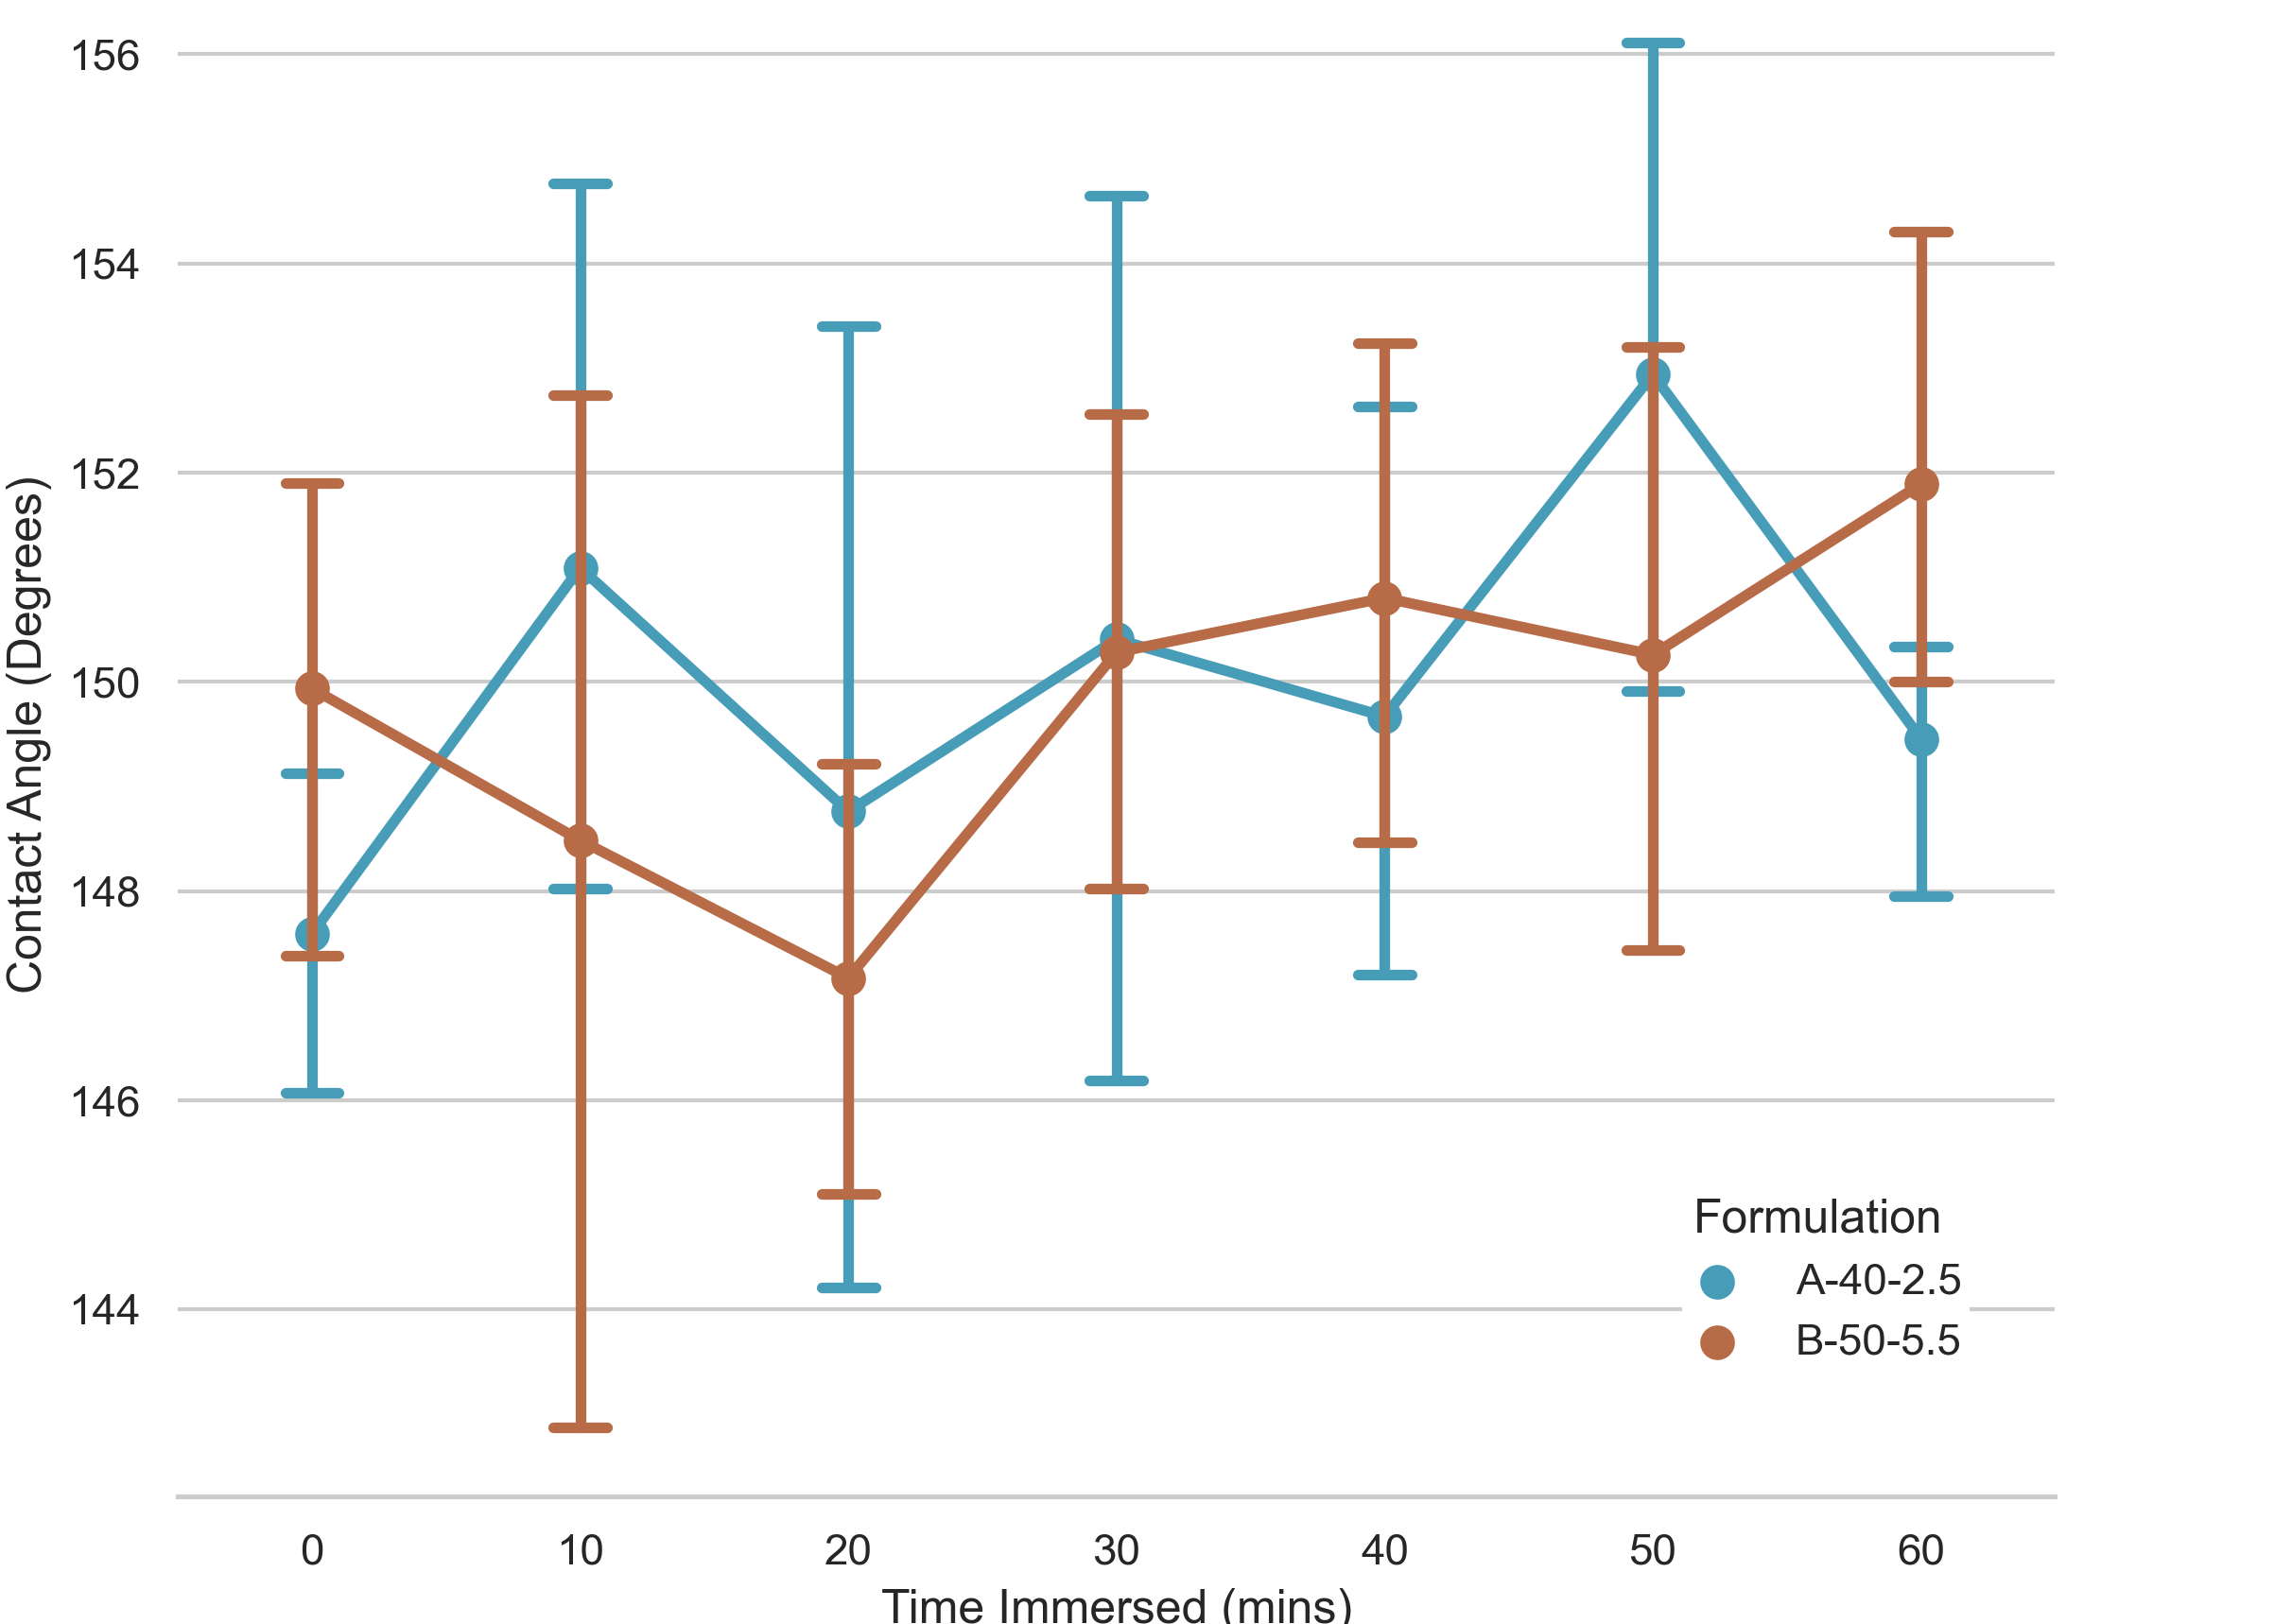
\includegraphics[width=0.43\textwidth]{Sections/Figures/Immersion3.png}
  \caption{Plot of Contact Angle as a function of time immersed in water for PE/Toluene and optimised formulation, showing standard deviation bars}\label{Immersion}
\end{figure} 
Figure \ref{Immersion} demonstrates that there was no statistically significant drop in hydrophobicity for either of the slides due to an overlap in the standard deviation bars. In addition, the formulations show no statistical difference \emph{between} each other at any time stamp. This further corroborates the conclusion that B-50-5.5 is a valid replacement for A in terms of super hydrophobicity and durability. 
\\ 
\par Nonetheless, a longer immersion time would be insightful as to the long-term effects of immersion. It can be concluded that both the B-50-5.5 and A-40-2.5 coatings show excellent hydrophobic durability up to 1 hour, with no statistically significant degradation,  however long term experiments are required to examine if a plateau has truly been reached. 

\begin{figure}[H]
\centering
\begin{subfigure}{.11\textwidth}
  \centering
  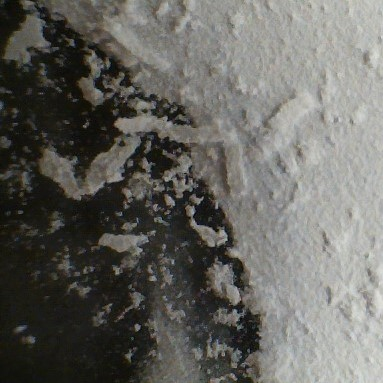
\includegraphics[width=1\linewidth]{Sections/Figures/A_Opt.jpg}
  \caption{A-40-2.5}
  \label{fig:sub1}
\end{subfigure}%
\begin{subfigure}{.11\textwidth}
  \centering
  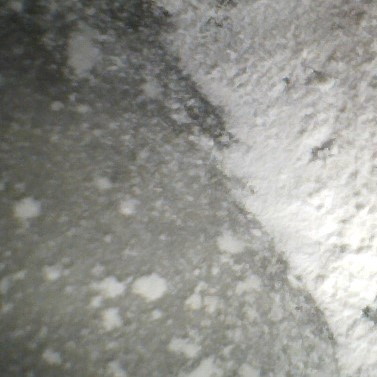
\includegraphics[width=1\linewidth]{Sections/Figures/B_opt.jpg}
  \caption{B-50-5.5}
  \label{fig:sub2}
\end{subfigure}
\caption{Images taken at 50X magnification}
\label{fig:test}
\label{abrased}
\end{figure}
\newpage

\par The average time recorded during \textbf{Mechanical Abrasion Testing} for 2 slides of 'A-40-2.5' and 'B-50-7.5' was 5.1 seconds and 5.7 seconds respectively. The disparity of 0.6 seconds suggests durability is comparable. Figure \ref{abrased} shows that A-40-2.5 formed a more coarse powder due to PE polymer grains. 
\par During \textbf{outdoor testing} 2 Slides of A-40-2.5 and 2 slides of B-50-5.5 were placed on the windowsill from 02-Dec-2020 to 07-Dec-2020 in SW7, London, UK. The average temperature was 5 °C $\pm$ 3°C with an RH of 90\%. Rain was recorded on 3 of the 5 days. 


%\begin{figure}[h!]
%\centering
%  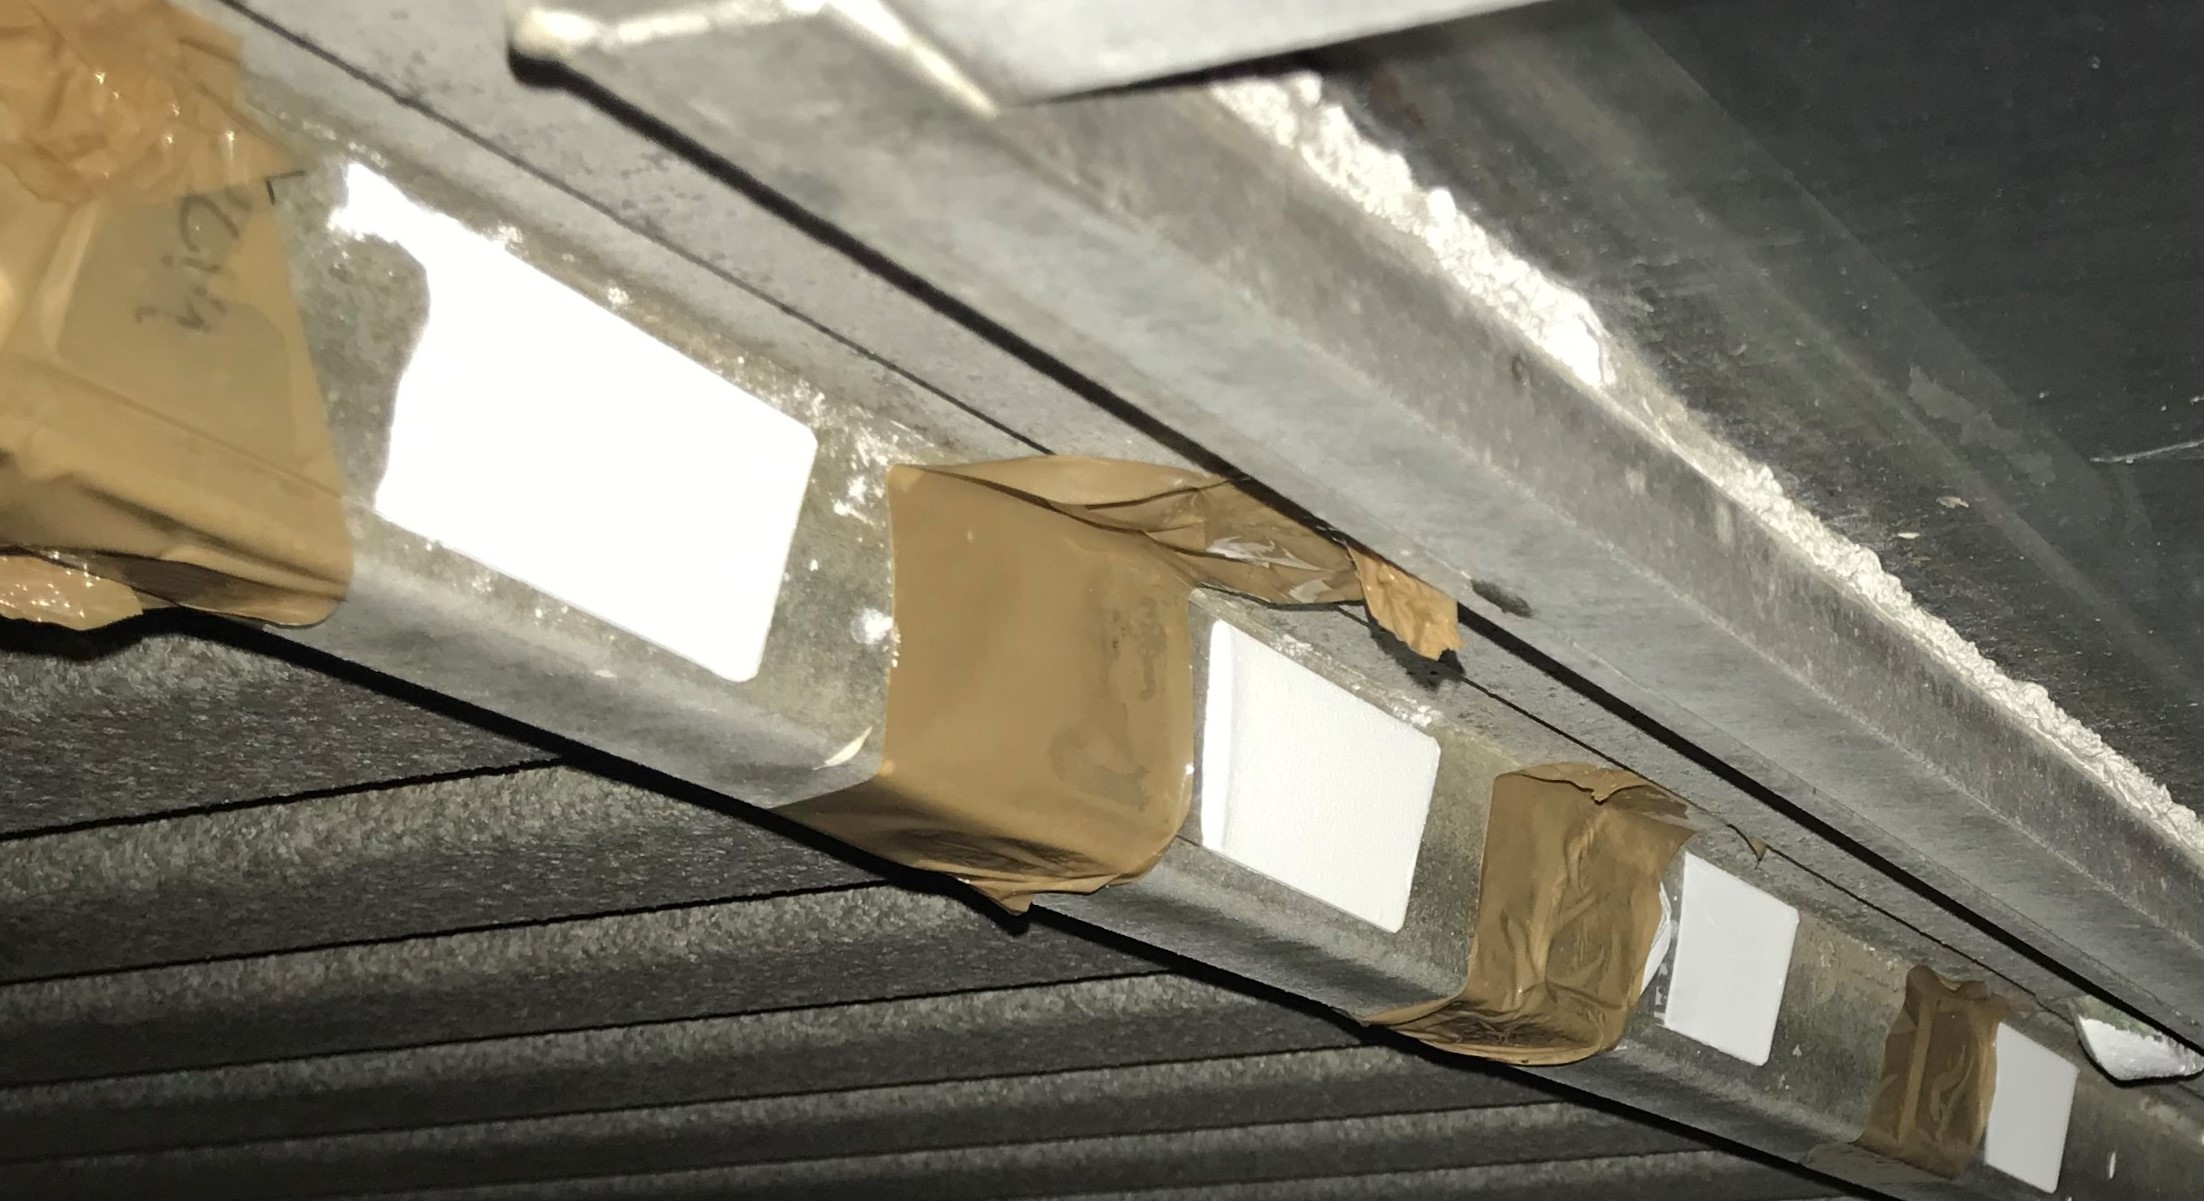
\includegraphics[width=0.2\textwidth]{Sections/Figures/Outdoor2.jpg}
%  \caption{The slides after 5 days of outdoor exposure on the windowsill with B-50-5.5 in the foreground of the image }\label{HPOpt}
%\end{figure}



\begin{table}[H]
\centering
\begin{tabular}{llr111}
\toprule


Description  & $\mu_1$    & $s_1$  & $\mu_2$    & $s_2$  & $t$   \\
\midrule
A-40-2.5 (1) & 152.8 & 3.9 & 147.6 & 1.9 & 2.0 \\ 
A-40-2.5 (2) & 150.1 & 1.1 & 149.7 & 1.1 & 0.4 \\ 
B-50-5.5 (1) & 151.8 & 2.9 & 146.5 & 3.6 & 1.9 \\ 
B-50-5.5 (2) & 151.6 & 1.8 & 150.9 & 2.5 & 0.4 \\ 
\bottomrule
\end{tabular}
\caption{1 is before and 2 is after the outdoor test. $\mu$ is the mean static WCA and $s$ is the sample standard deviation}
\end{table}
\begin{wrapfigure}{r}{0.23\textwidth}
\centering
    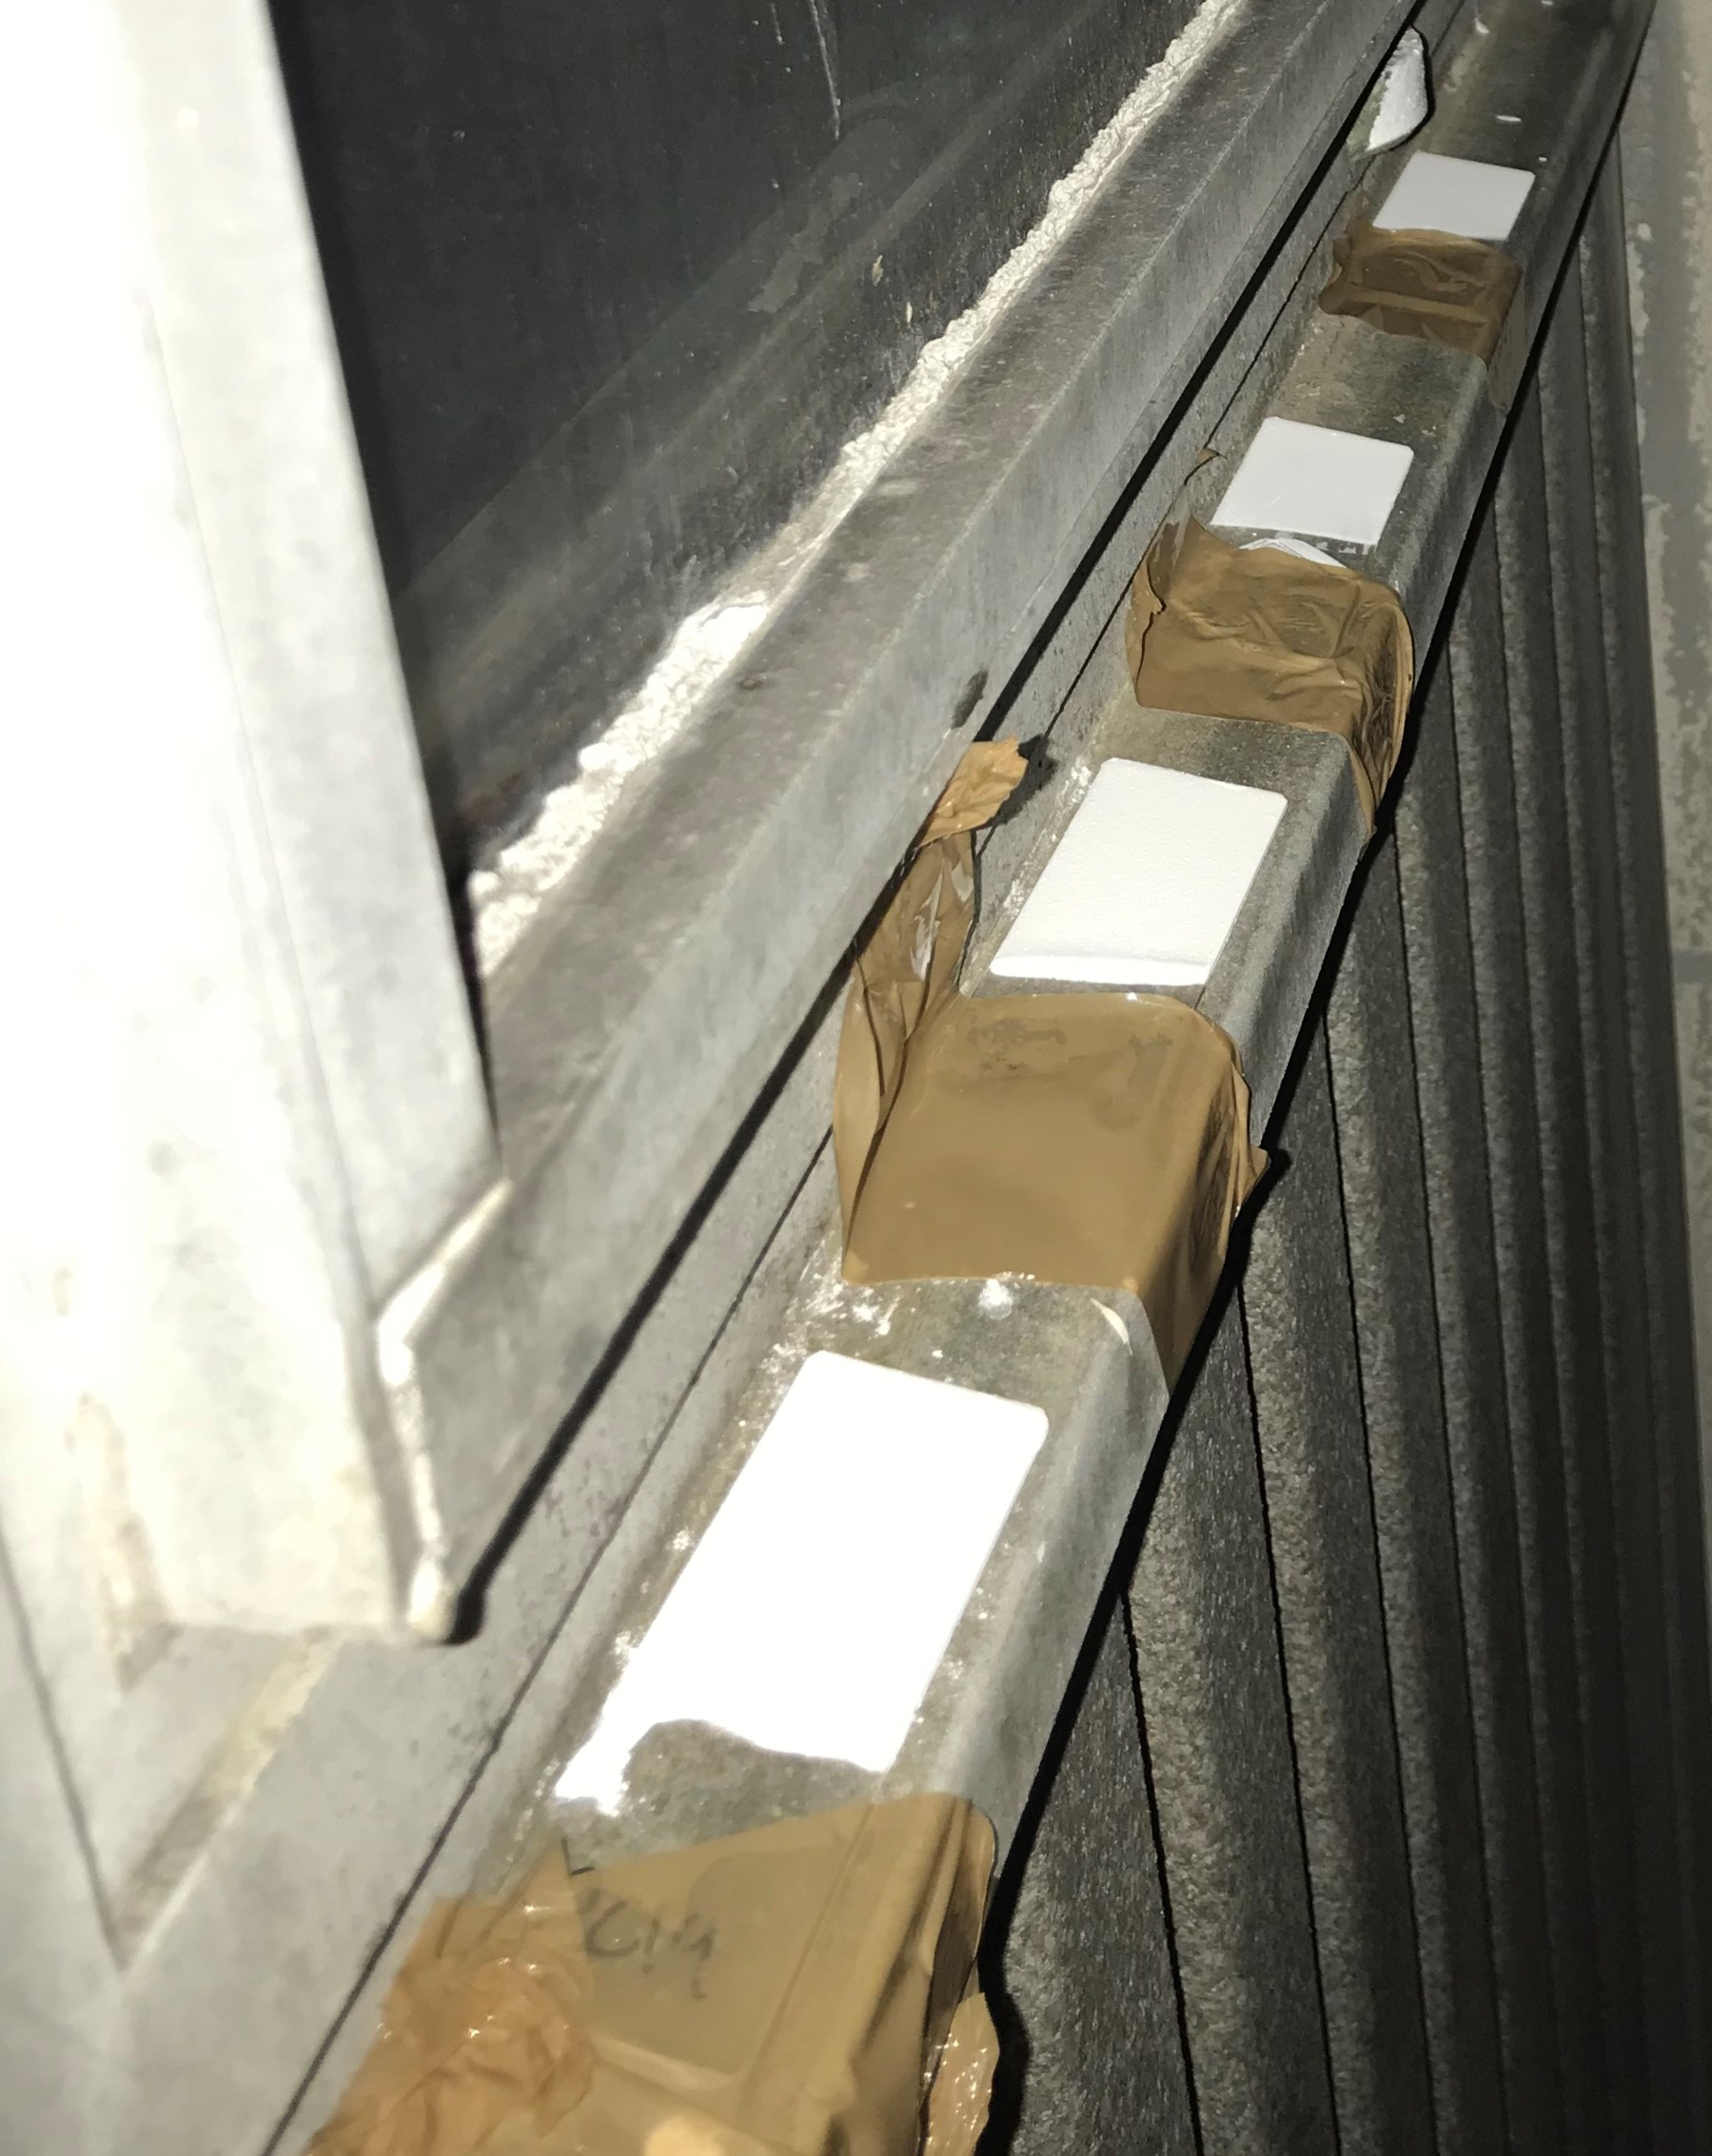
\includegraphics[width=0.09\textwidth]{Sections/Figures/Outdoor.jpg}
  \caption{ A-40-2.5 and B-50-5.5 placed on windowsill at SW7, UK}
  \label{Outdoor}
\end{wrapfigure}


A one-tailed t-test was used to test the hypothesis, at the 95\% significance level that there was no statistical difference before and after the outdoor test. $H_0: \mu_1 = \mu_2$ and $H_1: \mu_1 > \mu_2$. $\nu$ = 4 and so $t_c = 2.132$. Therefore, the null hypothesis was not rejected, and it was concluded that the integrity of both coatings was retained in outdoor conditions.





%------------------------------------------------
%\section{Discussion}
%Make sure this dscussion is NOT a description of Results

%“what do my results mean?”

%t should relate back directly to the questions posed in your introduction, and contextualize your results within the literature you have covered in your literature review. In order to make your discussion section engaging, you should include the following information:

%The major findings of your study
%The meaning of those findings
%How these findings relate to what others have done
%Limitations of your findings
%An explanation for any surprising, unexpected, or inconclusive %results
%Suggestions for further research

%Your discussion should NOT include any of the following %information:

%New results or data not presented previously in the paper
%Unwarranted speculation
%Tangential issues
%Conclusions not supported by your data



\section{Conclusion}
This paper built on previous work done by \cite{khoo_lim_2017}, \cite{Vatsal} \& \cite{Kokkinis_2017} by replacing the petrochemically derived materials with a biopolymer in corn starch. The modifications successfully produced comparable static and advancing contact angles to the PE/Toluene films in the optimised formulation:

\begin{table} [H]
\centering
\begin{tabular}{llr1}
\toprule
Formulation & Static CA ($^\circ$) & Adv. CA ($^\circ$)\\
\midrule
A-40-2.5   & 154.8 $\pm$ 4.7 & 156.0 $\pm$ 4.3              \\ 
B-50-5.5   & 151.7 $\pm$ 1.5    & 155.3 $\pm$ 3.9           \\ 
\bottomrule
\end{tabular}
\caption{Table comparing Static and Advancing ($\theta_A$) contact angles of previous and optimised formulations}
\label{Conc}
\end{table}
With comparable angles at a first glance, further statistical analysis on contact angles revealed stronger conclusions: B-50-5.5 exhibited no statistical difference in either contact angle when compared to A-40-2.5 and therefore it was a viable option for sustainable development of superhydrophobic films. Durability-wise, the hygroscopicity of starch remained a limitation in DVS experiments. However, there was an insignificant change in hydrophobicity witnessed during the outdoor test; practically, the films had no degradation in integrity or hydrophobicity during this time. Immersion testing further attested to the practical integrity of the films, showing no statistical degradation of films. Mechanical durability is decreased to a limited degree, however. Additionally, starch \emph{modifications} proved unsuccessful; OMS saw difficulty in continuous film formation and the hydrophobicity exhibited by TEOS was outmatched by the optimised formulation containing native corn starch.
Globally, despite the hydrophilic properties of corn starch, there is sufficient evidence to conclude that starch is a promising eco-binder to eliminate PE/Tol in the production of superhydrophobic films using hydrophobic calcium carbonate powder. 


%\begin{itemize}
%    \item Scope to use starch binder to replace A
%    \item Promising range of hydrophobic films and superhydrophobicity achieved through optimisation
%    \item Static angle reported for 'A-40-2.5' 154.8$^\circ$ ± 4.7 $^\circ$ and B-50-5.5 151.7 $^\circ$ ± 1.5 $^\circ$
%    \item Statistical analysis on advancing angles has strong conlusions - ANOVA test has shown that at least one of the starch formulations are different from the %'population' of starch formulations.  Proven by t-test B-50-5.5 statistically different to B-40-5.5 with 95\% certainty hence an optimum verified from Advancing contact %angle as well as static.
%    \item t-test between A-40-2.5 and B-50-5.5  proves we cannot reject null hypothesis and means that starch can be replaced from an advancing angle viewpoint. 
%    \item Hygroscopicity of starch remains a limitation but insignificant effect on hydrophobicity shown from the outdoor test. 
%    \item Outdoor testing has conclusive results, impressive performance considering derived from starch 
%    \item Mechanical durability is decreased to a limited degree, expected from starch comapred to PE. 
%    \item Elimianted toluene and plastic use, semi-renewable and can be combined with renewable sources of CaCO$_3$ such as eggshell so promising. 
%    \item Starch modifications were not successful due to the scientific nature of the report. Cannot change more than one variable, potentially with further scope a %modification can enhance film performance. 
%    \item 
%\end{itemize}

%Despite the properties of starch being heavily influence by water, there is sufficient evidence to conclude that starch is a  promising eco-binder to replace PE/Tol to produce superhydrophobic films using hydrophobic calcium carbonate powder. 

\section{Recommendations}
The results of this exploratory investigation provide strong evidence for further targeted research into the incorporation of starch into superhydrophobic films. Logically, replacing the PCC used with eggshell waste as done by \cite{khoo_lim_2017} should be the next step to further improve the sustainability credentials of the novel films developed in this investigation. Attempts to reduce the ethanol used in the formulation protocol, and thereby reduce VOC offgassing during drying,  will also help towards this goal. Additionally, a complete study of the hysteresis (namely $\theta_R$) using sliding, captive bubble or evaporation methods (\cite{eral}) should be undertaken to characterise the films further and further verify the optimised formulation presented here. To verify industrial applicability, characterisation using SEM, FTIR and TGA are required and investigations into alternative coating methods such as spin coating or bio-mineralisation (\cite{tang_chang_li_ge_niu_wang_jiang_sun_2021} will provide further insight into the real-world practicality of these film. More broadly, further starch modifications should be investigated to dampen its hydrophilicity; this includes cross-linking of polymers to occupy hydroxyl groups and etherification/esterification using different materials with the objective of increasing hydrophobicity and decreasing apparent hygroscopicity (\cite{wang}).  

%\begin{itemize}
%\item Biomneralization 
%\item crystallization 
%\item Ball milling to make more uniform powder \cite{fang_2019} rather than pestle mortar
%\item modified starches - use alkyl groups 
%\item Homogenization 
%\item Control Humidity 
%\item use of other surfactants with starch 
%\item Stearic acid - Vivian Consuelo Reolon Schmidt a et al. 
%\item cross- linking from hydrophobic modifications (\cite{wang} 
%\item Synthesis of transparent films \cite{rewritable}
%\item Changing substrate - silanization of glass to make films stick better.
%\item Investigate 2 phase separation of powder and binder due to differing surface energies. Eradicate with spray coating. 
%\item Improve hydrophobic and mechanical properties of starch films by addition of modified fillers. %https://www.sciencedirect.com/science/article/pii/S0141813019354066
%\item Thermal properties (TGA Analysis)
%\item FTIR (Test hydrophobic starches produced) 
%\item SEM (Surface Morphology and particle size of starch)
%\item The failure in measuring the WCA using the Sesile Drop method led us to want to adopt the the Captive bubble method, where the CA of a water-submerged air bubble underneath the test plate was measured following the protocol of Wu [24]. Or evaporation method. 
%\item A modification of the sessile drop method is the evaporation method [29, 32, 33], where the receding angle is measured as a droplet evaporates
%\item cellulose can be used as a replacement. 
%\end{itemize}
%\begin{itemize}
%\item Different concentrations of Ethanol to influence drying rate 
%\item Starch alternatives - we used modified starches that were less hydrophillic - less swelling i.e. OMS Alkyl modified
%\item different processes to reach starch gelatinization (mix longer?)
%\item different natural binder e.g. ethyl cellulose (swelling problem)
%\end{itemize}


\section{Acknowledgements}
We would like to express our sincere gratitude to \textbf{Dr Vikram A Karde} for his guidance throughout the project; \textbf{Dr Jerry Heng} for his kind assistance throughout the research; \textbf{Mr Ethan Errington} for assistance with training during unprecedented times. 



%----------------------------------------------------------------------------------------
%	REFERENCE LIST
%----------------------------------------------------------------------------------------

\begingroup
%\setstretch{0.7}
%\fontsize{4}{10}
\bibliography{references}
%\printbibliography
\endgroup




%----------------------------------------------------------------------------------------

\end{document}


%Maecenas sed ultricies felis. Sed imperdiet dictum arcu a egestas. 
%\begin{itemize}
%\item Donec dolor arcu, rutrum id molestie in, viverra sed diam
%\item Curabitur feugiat
%\item turpis sed auctor facilisis
%\item arcu eros accumsan lorem, at posuere mi diam sit amet tortor
%\item Fusce fermentum, mi sit amet euismod rutrum
%\item sem lorem molestie diam, iaculis aliquet sapien tortor non nisi
%\item Pellentesque bibendum pretium aliquet
%\end{itemize}
%\blindtext % Dummy text

%Text requiring further explanation\footnote{Example footnote}.

%------------------------------------------------